\documentclass[11pt]{article}

\usepackage[margin=1in, top=1.15in, bottom=1.15in]{geometry}

\usepackage{amsmath, amssymb, amsthm}

\usepackage{graphicx}
\usepackage{subcaption}
\usepackage{float}

\usepackage{microtype}
\usepackage{lmodern}

\usepackage[colorlinks=true, linkcolor=blue, citecolor=blue, urlcolor=blue]{hyperref}

\usepackage{natbib}
\bibliographystyle{plainnat}

\usepackage{booktabs}
\usepackage{enumitem}
\usepackage{xcolor}

\newcommand{\HH}{\mathbb{H}}
\newcommand{\CC}{\mathbb{C}}
\newcommand{\RR}{\mathbb{R}}
\newcommand{\dif}{\,\mathrm{d}}
\newcommand{\conj}[1]{\overline{#1}}
\newcommand{\abs}[1]{\left\lvert #1 \right\rvert}
\newcommand{\Imag}{\mathrm{Im}}
\newcommand{\Real}{\mathrm{Re}}

\newtheorem{theorem}{Theorem}
\newtheorem{proposition}[theorem]{Proposition}
\newtheorem{lemma}[theorem]{Lemma}
\newtheorem{remark}{Remark}

\begin{document}

\begin{titlepage}
  \centering
  \vspace*{3.5cm}
  {\LARGE\bfseries Ideal Fluid Flow in a Polygonal Domain\\[0.6em]
   via the Schwarz--Christoffel Transformation\par}
  \vspace{2.5cm}
  {\large
    Congyuan Zheng\\
    \small Dept.\ of Applied Mathematics \& Dept.\ of Geography,
    University of Colorado Boulder\\[1em]
    \large Sophia Arany\\
    \small Dept.\ of Applied Mathematics,
    University of Colorado Boulder\\[1em]
    \large Alexander Ingalls\\
    \small Dept.\ of Aerospace Engineering,
    University of Colorado Boulder\par}
  \vspace{2.5cm}
  {\normalsize APPM 4360, Complex Variables and Applications,
   Spring 2026\\[0.4em]
   April 27, 2026\par}
\end{titlepage}

\begin{abstract}
This paper applies the Schwarz--Christoffel (SC) conformal mapping to simulate
steady, irrotational, incompressible fluid flow inside the Boulder, Colorado
city-boundary polygon. The SC transformation maps the upper half-plane $\HH$
conformally onto the polygonal domain $\Omega$, converting analytically tractable
complex potentials in $\HH$ into physically meaningful streamline and equipotential
patterns in the physical domain. Four progressively enriched flow models are
implemented: (i)~uniform ideal flow, (ii)~terrain-corrected flow using USGS 3DEP
elevation data fitted by a thin-plate-spline radial basis function, (iii)~doubly-connected
flow with the downtown urban core modelled as an impenetrable obstacle via the
Milne-Thomson circle theorem, and (iv)~a road-vortex model placing point vortices
at major OSM road intersections. The SC parameter problem is solved via softmax
pre-vertex parameterisation and Levenberg--Marquardt least squares on side-length
ratios computed by Gauss--Legendre quadrature. All results are produced through
the forward SC map, yielding artifact-free streamlines and conformal grids that
satisfy the no-penetration boundary condition exactly by construction.
\end{abstract}

\newpage

\section{Introduction}

Computing fluid flow in an arbitrary domain is a hard problem: Laplace's equation
$\nabla^2\phi=0$ possesses no elementary closed-form solution in an irregular
geometry. The classical remedy, known since the 19th century, is conformal mapping.
A conformal map $z = f(\zeta)$ from a canonical domain (the unit disk or the upper
half-plane) to the physical region $\Omega$ transforms the Laplacian from one domain
to the other while preserving harmonicity. Any analytic function $W(\zeta)$ that
satisfies the required boundary conditions in the canonical domain automatically
produces a valid solution in $\Omega$, with zero grid-based discretization required.

The Schwarz--Christoffel (SC) transformation, developed independently by
H.~A.~Schwarz and E.~B.~Christoffel in the 1860s, provides an explicit integral
formula for the conformal map from the upper half-plane $\HH$ to any polygon.
For analytic polygons the parameter problem (choosing the pre-images of the
vertices on the real axis) can sometimes be solved in closed form; for general
$n$-gons it must be treated numerically. The modern numerical theory was
systematised by Driscoll and Trefethen~\citep{DT09}, who proved convergence of
parameter-problem algorithms and provided extensive software.

For polygonal physical domains, which arise naturally from administrative
boundaries, room layouts, channel cross-sections, and urban footprints, the
SC map provides exact, analytic access to the interior flow. This stands in
contrast to finite-element or finite-difference methods, which introduce
discretization error and require a mesh that conforms to the boundary.

The present project applies the SC transformation to the Boulder, Colorado
city-boundary polygon (a 1935-vertex TIGER/Line shape~\citep{TIGER25} simplified
to 11 vertices after Douglas--Peucker reduction and angle smoothing). We implement
the complete numerical pipeline from scratch in Python: polygon preprocessing,
the SC parameter problem, the forward map, and four physical potentials of
increasing complexity. The mathematical framework is drawn from
\citet{AF03,DT09}; the fluid-dynamics background from \citet{BO99} and
\citet{MT68}.

The four models are: (i)~\textit{uniform flow} $W=U\zeta$, providing the baseline
conformal streamline grid; (ii)~\textit{terrain-corrected flow} driven by USGS
elevation data modelled as distributed source/sink singularities in $\HH$;
(iii)~\textit{doubly-connected flow} in which the downtown commercial core acts
as an impenetrable obstacle, modelled via the Milne-Thomson circle theorem; and
(iv)~\textit{road-vortex flow} placing point vortices at major OSM road intersections
to capture local circulation. Each correction is additive in the complex potential
and preserves the no-penetration boundary condition on $\partial\Omega$ via the
method of images.

\paragraph{Organisation.}
Section~\ref{sec:theory} develops the SC mapping theory and complex-potential
framework, with full step-by-step derivations of every key result.
Section~\ref{sec:numerical} describes the numerical algorithms.
Section~\ref{sec:models} derives the four flow models. Section~\ref{sec:results}
presents the figures and discusses the results. Section~\ref{sec:conclusions}
summarises conclusions and future directions.

\section{Mathematical Framework}
\label{sec:theory}

\subsection{Ideal Fluid Flow and the Complex Potential}
\label{sec:ideal-flow}

A steady two-dimensional flow is \emph{ideal} when the velocity field
$\mathbf{u} = (u, v)$ satisfies two conditions simultaneously:
\begin{align}
  \text{irrotational:} \quad & \nabla \times \mathbf{u}
    = \frac{\partial v}{\partial x} - \frac{\partial u}{\partial y} = 0,
    \label{eq:irrotational}\\
  \text{incompressible:} \quad & \nabla \cdot \mathbf{u}
    = \frac{\partial u}{\partial x} + \frac{\partial v}{\partial y} = 0.
    \label{eq:incompressible}
\end{align}

\paragraph{Step 1: Velocity potential.}
Condition~\eqref{eq:irrotational} states that the curl of $\mathbf{u}$ vanishes.
In a simply connected region this forces $\mathbf{u}$ to be a gradient field:
there exists a scalar function $\phi(x, y)$, the \emph{velocity potential}, such
that
\begin{equation}
  \mathbf{u} = \nabla \phi, \qquad
  u = \frac{\partial \phi}{\partial x}, \quad
  v = \frac{\partial \phi}{\partial y}.
  \label{eq:velpot}
\end{equation}

\paragraph{Step 2: Laplace equation for $\phi$.}
Substituting~\eqref{eq:velpot} into~\eqref{eq:incompressible} gives
\begin{equation}
  \nabla \cdot \nabla \phi
  = \frac{\partial^2 \phi}{\partial x^2} + \frac{\partial^2 \phi}{\partial y^2}
  = \nabla^2 \phi = 0.
  \label{eq:laplace-phi}
\end{equation}
The velocity potential satisfies Laplace's equation throughout the flow domain.

\paragraph{Step 3: Stream function.}
Condition~\eqref{eq:incompressible} states that $\mathbf{u}$ has vanishing
divergence. In a simply connected region this forces $\mathbf{u}$ to be the
skew-gradient of a second scalar function $\psi(x, y)$, the \emph{stream
function}, defined by
\begin{equation}
  u = \frac{\partial \psi}{\partial y}, \qquad
  v = -\frac{\partial \psi}{\partial x}.
  \label{eq:streamdef}
\end{equation}
Direct substitution into $\nabla \cdot \mathbf{u}$ gives
$\partial_x (\partial_y \psi) - \partial_y (\partial_x \psi) = 0$ identically,
confirming that incompressibility is automatic.

\paragraph{Step 4: Laplace equation for $\psi$.}
Now apply irrotationality~\eqref{eq:irrotational} to~\eqref{eq:streamdef}:
\begin{equation}
  \frac{\partial v}{\partial x} - \frac{\partial u}{\partial y}
  = -\frac{\partial^2 \psi}{\partial x^2} - \frac{\partial^2 \psi}{\partial y^2}
  = -\nabla^2 \psi = 0,
\end{equation}
so the stream function also satisfies Laplace's equation,
$\nabla^2 \psi = 0$.

\paragraph{Step 5: Cauchy--Riemann equations.}
Comparing~\eqref{eq:velpot} and~\eqref{eq:streamdef} gives
\begin{equation}
  \frac{\partial \phi}{\partial x} = \frac{\partial \psi}{\partial y},
  \qquad
  \frac{\partial \phi}{\partial y} = -\frac{\partial \psi}{\partial x}.
  \label{eq:CR}
\end{equation}
These are exactly the Cauchy--Riemann equations for the complex function
\begin{equation}
  W(z) = \phi(x, y) + i\,\psi(x, y), \qquad z = x + iy,
  \label{eq:W}
\end{equation}
which means $W(z)$ is analytic on the flow domain $\Omega \subset \CC$. The pair
$(\phi, \psi)$ are \emph{harmonic conjugates}. The function $W$ is called the
\emph{complex potential}.

\paragraph{Step 6: Velocity from $W'(z)$.}
For any analytic function, the complex derivative can be computed along the
$x$-direction:
\begin{equation}
  W'(z) = \frac{\partial W}{\partial x}
  = \frac{\partial \phi}{\partial x} + i\,\frac{\partial \psi}{\partial x}.
\end{equation}
Using~\eqref{eq:velpot} and the second Cauchy--Riemann equation
$\partial_x \psi = -\partial_y \phi = -v$, we obtain
\begin{equation}
  W'(z) = u - i v = \overline{u + iv},
\end{equation}
so the Cartesian velocity components are recovered via
\begin{equation}
  (u, v) = \left(\Real W'(z),\ -\Imag W'(z)\right), \qquad
  \mathbf{u} = \overline{W'(z)}.
  \label{eq:velocity}
\end{equation}

\paragraph{Physical interpretation.}
Level curves of $\phi$ are \emph{equipotentials}; level curves of $\psi$ are
\emph{streamlines}. The gradient of $\phi$ gives the velocity, and by the
Cauchy--Riemann equations $\nabla \phi \cdot \nabla \psi = 0$, so streamlines
and equipotentials meet orthogonally wherever $W'(z) \neq 0$. The no-penetration
condition on a solid boundary $\partial \Omega$ reads
$\mathbf{u} \cdot \hat{\mathbf{n}} = 0$, which is equivalent to
$\psi = \mathrm{const}$ along $\partial \Omega$ (streamlines cannot cross the
boundary).

\subsection{Conformal Mapping Preserves Harmonicity}
\label{sec:conformal}

The reason conformal mapping works for ideal flow is captured by the following
classical identity.

\begin{lemma}[Conformal invariance of the Laplacian]
\label{lem:conformal}
Let $f : \HH \to \Omega$ be a bijective analytic map with $f'(\zeta) \neq 0$.
If $W(\zeta) = \phi(\xi, \eta) + i\,\psi(\xi, \eta)$ is analytic on $\HH$, then
$\tilde{W}(z) = W(f^{-1}(z))$ is analytic on $\Omega$, and its real and
imaginary parts satisfy $\nabla_z^2 \tilde{\phi} = 0$ and
$\nabla_z^2 \tilde{\psi} = 0$.
\end{lemma}

\begin{proof}[Sketch]
Composition of analytic functions is analytic, and analyticity implies the
Cauchy--Riemann equations, which in turn imply that both real and imaginary
parts solve Laplace's equation. Quantitatively, if $\zeta = f^{-1}(z)$ then
$\nabla_z^2 \tilde{\phi}(z) = \abs{(f^{-1})'(z)}^2\, \nabla_\zeta^2 \phi(\zeta)
= 0$.
\end{proof}

This is the key structural fact: any solution of Laplace's equation in $\HH$
pulls back to a solution in $\Omega$. The burden of the analysis is therefore
to find $f$ explicitly.

\subsection{The Riemann Mapping Theorem}

\begin{theorem}[Riemann, 1851]
\label{thm:riemann}
Let $\Omega \subsetneq \CC$ be a simply connected domain. There exists a
bijective conformal map $f : \HH \to \Omega$, unique up to post-composition
with a real M\"obius transformation of $\HH$.
\end{theorem}

The Boulder polygon is simply connected, so the theorem guarantees that a map
$f$ exists. The three real parameters of the M\"obius freedom correspond to
fixing three real pre-images on $\partial \HH = \RR \cup \{\infty\}$.

\subsection{The Schwarz--Christoffel Formula}
\label{sec:sc-formula}

For a polygon $\Omega$ with vertices $w_1, \dots, w_n$ (counter-clockwise) and
interior angles $\alpha_k \pi$, $\alpha_k \in (0, 2)$, the SC map takes the form
\begin{equation}
  f(\zeta) = A + C \int_{\zeta_0}^{\zeta}
    \prod_{k=1}^{n} (t - \zeta_k)^{\alpha_k - 1} \dif t,
  \label{eq:SC}
\end{equation}
where $\zeta_k \in \RR$ are the \emph{pre-vertices} (pre-images of $w_k$ on the
real axis), $A \in \CC$ is a translation, and $C \in \CC$ encodes scale and
rotation. The derivation of~\eqref{eq:SC} proceeds in four steps.

\paragraph{Step 1: Polygon angle sum identity.}
For a simple counter-clockwise polygon, the exterior angle at vertex $k$ (the
amount by which the tangent direction turns as we traverse the boundary through
$w_k$) is $\pi - \alpha_k \pi = \pi(1 - \alpha_k)$. The total exterior turning
over a full CCW traversal equals $2\pi$, hence
\begin{equation}
  \sum_{k=1}^{n} \pi(1 - \alpha_k) = 2\pi
  \quad\Longleftrightarrow\quad
  \sum_{k=1}^{n} \alpha_k = n - 2.
  \label{eq:anglesum}
\end{equation}

\paragraph{Step 2: Direction of $f'(\zeta)$ on the real axis.}
Take $\zeta = t$ real, $t \in (\zeta_k, \zeta_{k+1})$. For the factor
$(t - \zeta_j)^{\alpha_j - 1}$:
\begin{itemize}[leftmargin=2em, itemsep=0.25em]
  \item if $j \leq k$ (so $t > \zeta_j$), then $t - \zeta_j > 0$ is real and
        $\arg[(t - \zeta_j)^{\alpha_j - 1}] = 0$;
  \item if $j > k$ (so $t < \zeta_j$), then $t - \zeta_j < 0$ is real and
        $\arg[(t - \zeta_j)^{\alpha_j - 1}] = (\alpha_j - 1) \pi$
        (using the principal branch with $\arg(-1) = \pi$).
\end{itemize}
Therefore
\begin{equation}
  \arg f'(t) = \arg C + \sum_{j > k}^{n} (\alpha_j - 1) \pi
  = \arg C + \pi \sum_{j = k+1}^{n} (\alpha_j - 1).
  \label{eq:argfprime}
\end{equation}
This is constant on the open interval $(\zeta_k, \zeta_{k+1})$, so the image
$f((\zeta_k, \zeta_{k+1}))$ is a straight line segment, which is the $k$-th
edge of the polygon.

\paragraph{Step 3: Jump at each vertex.}
When $t$ crosses $\zeta_k$ from left to right, the factor $(t - \zeta_k)^{\alpha_k - 1}$
changes from a negative real base (argument $\pi$) to a positive real base
(argument $0$). The argument of $(t - \zeta_k)^{\alpha_k - 1}$ therefore decreases
by $(\alpha_k - 1) \pi$, which is an increase of $(1 - \alpha_k) \pi$. Since
$\arg f'$ gives the direction of the image edge, this jump is exactly the
exterior turning angle at vertex $w_k$, yielding an interior angle of
$\pi - (1 - \alpha_k) \pi = \alpha_k \pi$. This reproduces the prescribed polygon
geometry.

\paragraph{Step 4: Mapping is onto a bounded polygon.}
If $\zeta_n = \infty$ (one vertex is sent to infinity) the corresponding factor
$(t - \zeta_n)^{\alpha_n - 1}$ is dropped, and the integrand near infinity
behaves like $t^{\sum_{j<n}(\alpha_j - 1)} = t^{-\alpha_n - 1}$
(using~\eqref{eq:anglesum}), so the integral converges at infinity provided
$\alpha_n > 0$. Translating by $A$ places the polygon at the desired location;
multiplying by $C$ sets the overall scale and orientation.

\paragraph{Interior-angle computation in practice.}
Given vertices $w_0, \dots, w_{n-1}$ (complex, CCW), the two adjacent edge
vectors at $w_k$ are $\vec{e}_{k-1} = w_k - w_{k-1}$ (incoming) and
$\vec{e}_k = w_{k+1} - w_k$ (outgoing). The exterior turning angle (signed,
CCW positive) is
\begin{equation}
  \theta_k^{\mathrm{ext}}
  = \arg\!\left( \frac{w_{k+1} - w_k}{w_k - w_{k-1}} \right),
\end{equation}
and the interior angle in units of $\pi$ is therefore
\begin{equation}
  \alpha_k = 1 - \frac{1}{\pi}\,
    \arg\!\left( \frac{w_{k+1} - w_k}{w_k - w_{k-1}} \right),
  \label{eq:alpha}
\end{equation}
with indices modulo $n$. One verifies~\eqref{eq:anglesum} by summing: the
total exterior turning is $2\pi$.

\subsection{M\"obius Normalisation and the Parameter Problem}

The real M\"obius group $\mathrm{PSL}(2, \RR)$, acting on $\HH$ via
$\zeta \mapsto (a\zeta + b)/(c\zeta + d)$ with $ad - bc = 1$ and real
$a, b, c, d$, has three real parameters. We can therefore fix three of the
$n$ pre-vertices at prescribed real values without loss of generality. A
convenient choice in the normalised unit-interval parameterisation is
\begin{equation}
  \zeta_0 = -1, \qquad \zeta_1 = 0, \qquad \zeta_{n-1} = 1,
\end{equation}
leaving $n - 3$ free parameters $\zeta_2, \dots, \zeta_{n-2} \in (0, 1)$
subject to the ordering constraint $\zeta_2 < \zeta_3 < \cdots < \zeta_{n-2}$.
For Boulder's 11-vertex polygon, $n - 3 = 8$ free pre-vertices remain.

\subsection{Method of Images and Boundary Conditions}
\label{sec:images}

Any analytic function $W(\zeta)$ with $\Imag(W(\zeta)) = 0$ on $\zeta \in \RR$
automatically satisfies $\psi = 0$ on $\partial \HH$. Pulled back via the
conformal map $f$, this becomes $\psi = 0$ on $\partial \Omega$, i.e., the
no-penetration condition on the Boulder boundary.

\paragraph{Image construction.}
To add a singularity at $s = a + ib \in \HH$ (with $b > 0$) while preserving
$\Imag(W) = 0$ on the real axis, we add a mirror-image singularity at
$\bar{s} = a - ib$. For a source of strength $Q > 0$ at $s$, the image-pair
potential is
\begin{equation}
  W_{\mathrm{source}}(\zeta)
  = \frac{Q}{2\pi} \bigl[ \log(\zeta - s) + \log(\zeta - \bar{s}) \bigr].
  \label{eq:source-pair}
\end{equation}

\paragraph{Algebraic verification.}
We show $\Imag(W_{\mathrm{source}}) = 0$ on the real axis by direct computation.
Take $\zeta = x \in \RR$:
\begin{align}
  \log(x - s) &= \log(x - a - ib)
    = \tfrac{1}{2} \log\!\bigl[(x - a)^2 + b^2\bigr]
      + i\,\arg(x - a - ib),\\
  \log(x - \bar{s}) &= \log(x - a + ib)
    = \tfrac{1}{2} \log\!\bigl[(x - a)^2 + b^2\bigr]
      + i\,\arg(x - a + ib).
\end{align}
Adding:
\begin{equation}
  \log(x - s) + \log(x - \bar{s})
  = \log\!\bigl[(x - a)^2 + b^2\bigr]
    + i\,\bigl[\arg(x - a - ib) + \arg(x - a + ib)\bigr].
\end{equation}
The numbers $x - a - ib$ and $x - a + ib$ are complex conjugates, so their
arguments are opposite in sign:
$\arg(x - a - ib) = -\arg(x - a + ib)$. The bracketed imaginary part
therefore equals zero, giving
\begin{equation}
  \Imag\!\bigl[\log(x - s) + \log(x - \bar{s})\bigr]
  = 0 \quad \text{for all } x \in \RR. \qed
\end{equation}
The same cancellation applies to a point vortex of strength $\Gamma$, with
the coefficient $Q/(2\pi)$ replaced by $-i\Gamma/(2\pi)$, because the
logarithm pair cancels identically on the real axis regardless of the
(complex) multiplier.

\subsection{Point Vortex Potential}
\label{sec:vortex}

A point vortex of circulation $\Gamma$ located at $\zeta_0$ has complex potential
\begin{equation}
  W_{\mathrm{vortex}}(\zeta)
  = \frac{-i\,\Gamma}{2\pi} \log(\zeta - \zeta_0).
  \label{eq:vortex}
\end{equation}
We derive this from the definition of circulation and the complex-velocity
identity~\eqref{eq:velocity}.

\paragraph{Derivation.}
The velocity is
\begin{equation}
  W_{\mathrm{vortex}}'(\zeta) = \frac{-i\,\Gamma}{2\pi (\zeta - \zeta_0)}.
\end{equation}
Setting $\zeta - \zeta_0 = r e^{i\theta}$ (polar coordinates centred on
$\zeta_0$):
\begin{equation}
  W'(\zeta)
  = \frac{-i\,\Gamma}{2\pi r} e^{-i\theta}
  = \frac{\Gamma}{2\pi r}\, e^{-i(\theta + \pi/2)}.
\end{equation}
Using~\eqref{eq:velocity}, $\mathbf{u} = \overline{W'}$ has magnitude
$\abs{\mathbf{u}} = \Gamma / (2\pi r)$ and direction angle $\theta + \pi/2$,
which is perpendicular to the radial vector. The flow therefore consists of
concentric circular streamlines centred on $\zeta_0$. Computing the circulation
along the circle $\zeta - \zeta_0 = r e^{i\theta}$, $\theta \in [0, 2\pi]$:
\begin{equation}
  \oint \mathbf{u} \cdot \mathrm{d}\boldsymbol{\ell}
  = \int_0^{2\pi} \frac{\Gamma}{2\pi r} \cdot r\, \mathrm{d}\theta
  = \Gamma,
\end{equation}
confirming that $\Gamma$ is the circulation, as advertised.

\subsection{Milne-Thomson Circle Theorem}
\label{sec:MT}

\begin{theorem}[Milne-Thomson, 1940]
\label{thm:MT}
Let $W_0(\zeta)$ be an analytic complex potential with no singularities inside
the disk $D = \{\zeta : \abs{\zeta - \zeta_0} \leq a\}$. Then the potential
\begin{equation}
  W(\zeta) = W_0(\zeta)
  + \conj{W_0\!\left(\zeta_0 + \frac{a^2}{\conj{\zeta - \zeta_0}}\right)}
  \label{eq:MT}
\end{equation}
is analytic outside $D$ and has the circle $\partial D = \{\abs{\zeta - \zeta_0} = a\}$
as a streamline, i.e., $\psi = \Imag(W) = \mathrm{const}$ on $\partial D$.
\end{theorem}

\begin{proof}
We show directly that $W(\zeta)$ is real on $\partial D$. Write
$\zeta - \zeta_0 = a e^{i\theta}$ so that $\abs{\zeta - \zeta_0} = a$. Then
\begin{equation}
  \conj{\zeta - \zeta_0} = a e^{-i\theta}, \qquad
  (\zeta - \zeta_0)(\conj{\zeta - \zeta_0}) = a^2.
  \label{eq:circle-id}
\end{equation}
From~\eqref{eq:circle-id}:
\begin{equation}
  \frac{a^2}{\conj{\zeta - \zeta_0}}
  = \frac{(\zeta - \zeta_0)(\conj{\zeta - \zeta_0})}{\conj{\zeta - \zeta_0}}
  = \zeta - \zeta_0.
\end{equation}
Therefore on $\partial D$:
\begin{equation}
  \zeta_0 + \frac{a^2}{\conj{\zeta - \zeta_0}}
  = \zeta_0 + (\zeta - \zeta_0) = \zeta.
\end{equation}
Substituting into~\eqref{eq:MT}:
\begin{equation}
  W(\zeta) = W_0(\zeta) + \conj{W_0(\zeta)}
  = 2\,\Real\!\bigl[W_0(\zeta)\bigr]
  \in \RR.
\end{equation}
Hence $\Imag(W(\zeta)) = 0$ on $\partial D$, so $\partial D$ is a streamline. The
function in the second term of~\eqref{eq:MT} is the composition of $W_0$ with
the M\"obius-like inversion $\zeta \mapsto \zeta_0 + a^2/\conj{\zeta - \zeta_0}$,
which maps the exterior of $D$ to its interior. Because $W_0$ has no
singularities inside $D$, the composed function has no singularities in the
exterior of $D$. Taking the complex conjugate of the whole expression
preserves analyticity (in $\zeta$ rather than $\bar{\zeta}$) on the exterior;
a more careful argument uses the Schwarz reflection principle~\citep[Ch.~6]{MT68}.
\end{proof}

\paragraph{Specialisation to uniform flow.}
For $W_0(\zeta) = U \zeta$, we have
\begin{equation}
  W_0\!\left(\zeta_0 + \frac{a^2}{\conj{\zeta - \zeta_0}}\right)
  = U \zeta_0 + \frac{U a^2}{\conj{\zeta - \zeta_0}}.
\end{equation}
Taking the complex conjugate of the whole expression:
\begin{equation}
  \conj{U \zeta_0 + \frac{U a^2}{\conj{\zeta - \zeta_0}}}
  = \conj{U \zeta_0} + \frac{U a^2}{\zeta - \zeta_0}
  = \conj{U}\, \conj{\zeta_0} + \frac{U a^2}{\zeta - \zeta_0}.
\end{equation}
For real $U$ the first term is a constant which does not affect streamlines,
and in the upper-half-plane formulation we also add the image-pair
$U a^2 / (\bar{\zeta} - \bar{\zeta}_0)$ to satisfy the no-penetration condition
on the real axis. The final working expression is
\begin{equation}
  W_{\mathrm{urban}}(\zeta) = U \zeta
    + \frac{U a^2}{\zeta - \zeta_0}
    + \frac{U a^2}{\bar{\zeta} - \bar{\zeta}_0}.
  \label{eq:urban}
\end{equation}
The first additional term enforces $\psi = \mathrm{const}$ on the disk; the second
term restores $\psi = 0$ on $\RR$ by the method of images.

\section{Numerical Implementation}
\label{sec:numerical}

\subsection{Polygon Preprocessing}

The raw Boulder TIGER/Line boundary has 1935 vertices. SC solvers become
numerically unstable for $n\gtrsim 20$ due to \emph{SC crowding}: when a vertex
has an interior angle close to $0$ or $2\pi$, its pre-vertex $\zeta_k$ is
forced extremely close to a neighbor, causing catastrophic cancellation in the
quadrature integrals. Two preprocessing steps address this.

First, Douglas--Peucker simplification with an adaptive binary-search tolerance
(target: $10$--$16$ vertices) reduces the boundary to $\approx 14$ vertices.
Second, vertices whose interior angle falls outside $[0.35\pi, 1.75\pi]$ are
removed iteratively (one worst offender per pass), joining adjacent edges into
a single segment. Boulder converges to $\mathbf{11}$ vertices after this
angle-smoothing step. The polygon is then normalised to $O(1)$ scale and centred
at the origin for numerical stability.

\subsection{The SC Parameter Problem}
\label{sec:param}

The $n - 3$ free pre-vertices $\zeta_2, \dots, \zeta_{n-2} \in (0, 1)$ must be
chosen so that the image polygon $f(\RR)$ has the correct side-length ratios.
Define the $k$-th side length
\begin{equation}
  L_k = \abs{\, \int_{\zeta_k}^{\zeta_{k+1}}
    \prod_{j=1}^{n} (t - \zeta_j)^{\alpha_j - 1} \dif t \,},
\end{equation}
with indices taken modulo $n$ and the last side wrapping through $\pm \infty$.
The parameter problem requires matching $n - 1$ side-length ratios to the
target polygon:
\begin{equation}
  \frac{L_k}{L_{n-1}}
  = \frac{\abs{w_{k+1} - w_k}}{\abs{w_0 - w_{n-1}}},
  \quad k = 0, \dots, n - 2.
  \label{eq:param}
\end{equation}

\subsubsection{Softmax reparameterisation.}
\label{sec:softmax}

The constraint $0 < \zeta_2 < \zeta_3 < \cdots < \zeta_{n-2} < 1$ is awkward
for black-box optimisers, since a naive step can send a parameter outside the
feasible interval or violate the ordering. We therefore reparameterise via the
softmax of an unconstrained vector $p \in \RR^{n-3}$. Define
\begin{equation}
  w_j(p) = \frac{e^{p_j}}{\displaystyle\sum_{i=1}^{n-3} e^{p_i} + 1},
  \qquad j = 1, \dots, n - 3,
  \label{eq:softmax}
\end{equation}
and take a cumulative sum:
\begin{equation}
  \zeta_{k+1} = \sum_{j=1}^{k} w_j(p),
  \qquad k = 1, \dots, n - 3.
  \label{eq:cumsum}
\end{equation}

\paragraph{Derivation: positivity, ordering, and the box constraint.}
We verify that~\eqref{eq:softmax}--\eqref{eq:cumsum} automatically satisfy
all constraints.
\begin{enumerate}[leftmargin=2em]
\item \textit{Positivity.} Since $e^{p_i} > 0$ for all real $p_i$, each weight
  $w_j > 0$. Therefore the cumulative sums are strictly increasing:
  $\zeta_2 < \zeta_3 < \cdots < \zeta_{n-2}$.

\item \textit{Upper bound.} Let $S = \sum_{i=1}^{n-3} e^{p_i}$. Then
  $\sum_{j=1}^{n-3} w_j = S / (S + 1) < 1$, so every $\zeta_k \leq \sum_j w_j < 1$.

\item \textit{Lower bound.} The first cumulative partial sum is $\zeta_2 = w_1 > 0$.
\end{enumerate}
Thus for any $p \in \RR^{n-3}$ the pre-vertices $\zeta_2, \dots, \zeta_{n-2}$
land in the open interval $(0, 1)$ in strictly increasing order, converting a
constrained optimisation into an unconstrained one.

\subsubsection{Levenberg--Marquardt least squares.}

System~\eqref{eq:param} is solved by Levenberg--Marquardt (LM), accessed via
\texttt{scipy.optimize.least\_squares} with \texttt{method=`lm'} and up to
$18{,}000$ function evaluations. Given a residual vector
$r(p) \in \RR^{n-1}$ (the difference between computed and target side-length
ratios), the LM update at iteration $t$ is
\begin{equation}
  p^{(t+1)} = p^{(t)}
    - \bigl( J^\top J + \lambda_t\, \mathrm{diag}(J^\top J) \bigr)^{-1}
      J^\top r(p^{(t)}),
\end{equation}
where $J$ is the Jacobian of $r$ with respect to $p$, and $\lambda_t$ is an
adaptive damping parameter. When $\lambda_t \to 0$ the update reduces to the
Gauss--Newton step (fast second-order convergence near a good solution); when
$\lambda_t \to \infty$ the update reduces to a small gradient-descent step
(stable near ill-conditioned regions). LM chooses $\lambda_t$ adaptively based
on whether the previous step reduced the cost.

This blending makes LM much more robust than either pure Gauss--Newton or
gradient descent in the presence of \emph{SC crowding}, where the Jacobian
becomes nearly singular along directions that pull crowded pre-vertices apart.

\subsubsection{Gauss--Legendre quadrature of the SC integral.}

Each side-length integral $L_k$ is evaluated by $N = 500$-node Gauss--Legendre
(GL) quadrature. The standard GL rule approximates
\begin{equation}
  \int_{-1}^{1} g(u) \dif u
  \approx \sum_{i=1}^{N} w_i\, g(u_i),
\end{equation}
where $u_i$ are the roots of the Legendre polynomial $P_N$ and $w_i$ are the
associated quadrature weights. The integral over $[\zeta_k, \zeta_{k+1}]$ is
mapped to $[-1, 1]$ via the affine change of variables
$t = \tfrac{1}{2}(\zeta_{k+1} - \zeta_k)\, u + \tfrac{1}{2}(\zeta_{k+1} + \zeta_k)$:
\begin{equation}
  \int_{\zeta_k}^{\zeta_{k+1}} g(t)\, \dif t
  = \frac{\zeta_{k+1} - \zeta_k}{2}
    \int_{-1}^{1} g\!\left(
      \tfrac{1}{2}(\zeta_{k+1} - \zeta_k)\, u
      + \tfrac{1}{2}(\zeta_{k+1} + \zeta_k)
    \right) \dif u.
\end{equation}
For smooth integrands GL converges exponentially in $N$, so $N = 500$ yields
essentially machine-precision accuracy. Crucially, the nodes $u_i$ and weights
$w_i$ are pre-computed once and reused across all LM iterations, reducing each
integral evaluation to a single vectorised dot product.

\subsubsection{Determining $A$ and $C$.}

Once the pre-vertices are known, the constants $A, C \in \CC$ are determined
by an overdetermined linear least-squares fit. For each vertex $w_k$, denote
by $I_k$ the SC integral from a reference point $\zeta_{\mathrm{ref}} = 0.5i$
to $\zeta_k + \varepsilon$ (where $\varepsilon$ is a small complex offset to
avoid the branch point). The linear system
\begin{equation}
  A + C \cdot I_k = w_k, \quad k = 0, 1, \dots, n - 1,
\end{equation}
has $n$ complex (equivalently, $2n$ real) equations in four real unknowns
$(\Real A, \Imag A, \Real C, \Imag C)$. The least-squares solution is computed
via \texttt{numpy.linalg.lstsq}.

\subsection{Forward Map and Streamline Computation}

All flow results are produced via the \emph{forward-map} approach, avoiding
Newton iterations on $f^{-1}$ for every pixel. A dense $400 \times 400$ grid of
$\zeta$ values in $\HH$ is mapped forward to $z = f(\zeta)$, each SC integral
evaluated by a $400$-node GL rule along an L-shaped path in $\HH$ that clears
the real-axis branch cuts. The complex potential $W(\zeta)$ is evaluated
analytically at each $\zeta$ point. The resulting scattered pairs
$(z_i, W(\zeta_i))$ are then interpolated onto a regular physical-plane grid by
\texttt{scipy.interpolate.griddata} (linear method). Streamlines
$\Imag(W) = \mathrm{const}$ and equipotentials $\Real(W) = \mathrm{const}$ are
extracted by standard contour-finding.

\paragraph{Topological note on closed streamlines.}
A subtle structural consequence of the forward-map SC picture deserves explicit
comment. Uniform flow in $\HH$ has streamlines $\Imag(\zeta) = \eta_0$, which
are horizontal lines running from $\zeta \to -\infty$ to $\zeta \to +\infty$.
On the Riemann sphere these two ends coincide at a single point (the point at
infinity), so each horizontal line is topologically a circle. The SC map sends
that single point to one fixed vertex on $\partial \Omega$. Every streamline
therefore becomes a closed curve inside $\Omega$, producing a circulatory flow
pattern rather than a crossing one.

This is a topological necessity of conformal mapping from $\HH$ onto a bounded
polygon, not a numerical artefact. Obtaining crossing streamlines that enter
one side of $\Omega$ and exit another requires either (a) relabelling the
polygon so that the "infinite side" spans opposite boundaries of $\Omega$,
or (b) switching the potential to a source-sink pair
$W = U \log[(\zeta - \zeta_{\mathrm{src}}) / (\zeta - \zeta_{\mathrm{sink}})]$
whose streamlines run from source to sink.

\paragraph{Why forward mapping.}
The alternative (inverse mapping) would require solving $f(\zeta) = z$ for
$\zeta$ at every pixel of the physical domain, which costs a full Newton
iteration per pixel. The forward approach evaluates $f(\zeta)$ once per grid
point in $\HH$, then uses Delaunay-based interpolation to recover values on a
regular physical grid. Grid points in $\HH$ map strictly inside the polygon by
construction, so the interpolated field is automatically zero outside $\Omega$,
yielding smooth boundary contours.

\section{Physical Flow Models}
\label{sec:models}

\subsection{Uniform Ideal Flow}

In $\HH$, uniform rightward flow of speed $U$ has the trivial complex potential
$W(\zeta) = U \zeta$. Streamlines are horizontal lines $\Imag(\zeta) = \eta_0$
and equipotentials are vertical lines $\Real(\zeta) = \xi_0$. Pulling back
through $f$ yields a conformal grid in $\Omega$; the Cauchy--Riemann
equations~\eqref{eq:CR} guarantee that streamlines and equipotentials remain
orthogonal wherever $f'(\zeta) \neq 0$.

\subsection{Terrain-Corrected Flow}
\label{sec:terrain}

Boulder's terrain drops approximately 480\,m from west ($\sim 2057$\,m) to east
($\sim 1576$\,m). Topographic slope drives a wind-speed component that acts as a
source (uphill face) or sink (downhill face) at each boundary segment. We model
this by one source/sink singularity per polygon vertex in $\HH$:
\begin{equation}
  W_{\mathrm{terrain}}(\zeta) = U \zeta
    + \sum_{k=1}^{n} \frac{Q_k}{2\pi}
      \bigl[ \log(\zeta - s_k) + \log(\zeta - \bar{s}_k) \bigr],
  \label{eq:terrain}
\end{equation}
where $s_k = \zeta_k + \delta i$ ($\delta = 0.25$) lifts the singularity into
$\HH$, and the image term $\log(\zeta - \bar{s}_k)$ preserves $\psi = 0$ on
$\RR$ by the cancellation of Section~\ref{sec:images}. The strength
$Q_k \propto (\nabla e)_k \cdot \hat{\mathbf{e}}_{\mathrm{flow}}$ is proportional
to the local elevation gradient projected onto the east-facing flow direction.

Elevation data is obtained from the USGS 3DEP EPQS API~\citep{USGS3DEP} at
$\approx 81$ sample points (polygon vertices, three interpolation points per
edge, and 25 interior grid points), fitted by a thin-plate-spline radial basis
function; 5-fold cross-validation gives $R^2 \approx 0.60$ for this run.
Per-vertex gradients are computed by centred finite differences ($h = 100$\,m)
on the RBF surface.

\subsection{Urban Obstacle: Doubly-Connected Domain}
\label{sec:urban-model}

The downtown commercial core introduces an interior obstacle, making $\Omega$
doubly connected. Applying $f^{-1}$ to the obstacle boundary yields a closed
curve $C \subset \HH$, bounded by its minimum enclosing circle (computed by
Welzl's algorithm~\citep{Welzl91}): centre $\zeta_0 \in \HH$, radius $a$. The
Milne-Thomson theorem of Section~\ref{sec:MT} then gives the closed-form
potential~\eqref{eq:urban}:
\begin{equation*}
  W_{\mathrm{urban}}(\zeta) = U \zeta
    + \frac{U a^2}{\zeta - \zeta_0}
    + \frac{U a^2}{\bar{\zeta} - \bar{\zeta}_0}.
\end{equation*}
The approximation error in treating the actual obstacle boundary as a circle is
$O((a / \Imag\, \zeta_0)^2)$. The achieved ratio for this run is
$\Imag(\zeta_0) / a = 5.36$, giving an approximation error of approximately
$3.5\%$.

\subsection{Road-Vortex Flow}
\label{sec:road}

Major road intersections generate local circulation in urban atmospheric flow
through traffic-induced turbulence and building channelling. We model each of
the $M$ highest-degree OSM road intersections inside $\Omega$ as a point vortex
in $\HH$. The physical intersection position $z_k^* \in \Omega$ is mapped to
$s_k \in \HH$ via Newton iteration on $f$ (SC inverse map). Using the single-vortex
potential~\eqref{eq:vortex} together with the method-of-images pairing, the
combined complex potential is
\begin{equation}
  W_{\mathrm{road}}(\zeta) = U \zeta
  + \sum_{k=1}^{M} \frac{-i\,\Gamma_k}{2\pi}
    \bigl[ \log(\zeta - s_k) + \log(\zeta - \bar{s}_k) \bigr],
  \label{eq:road}
\end{equation}
where $\Gamma_k \propto \deg(k)$ is proportional to the node degree (the number
of road arms meeting at intersection $k$). The sign convention is $\Gamma_k > 0$
(CCW) for intersections north of the polygon centroid and $\Gamma_k < 0$ (CW)
for those south, producing a vortex-pair shear consistent with Boulder's
prevailing westerly flow. The image term preserves $\psi = 0$ on $\RR$ via the
same cancellation used for the source pair in Section~\ref{sec:images}.

\section{Results}
\label{sec:results}

\subsection{Boulder Polygon Simplification}

Figure~\ref{fig:poly} shows the original 1935-vertex TIGER/Line boundary of
Boulder alongside the 11-vertex polygon used in the SC computation. The
Douglas--Peucker simplification removes the fine-scale boundary undulations
while preserving the essential east-west elongation and the northern
indentation that constitutes the most prominent geometric feature. The
simplified polygon is the actual domain $\Omega$ for all flow computations
that follow.

\begin{figure}[tp]
  \centering
  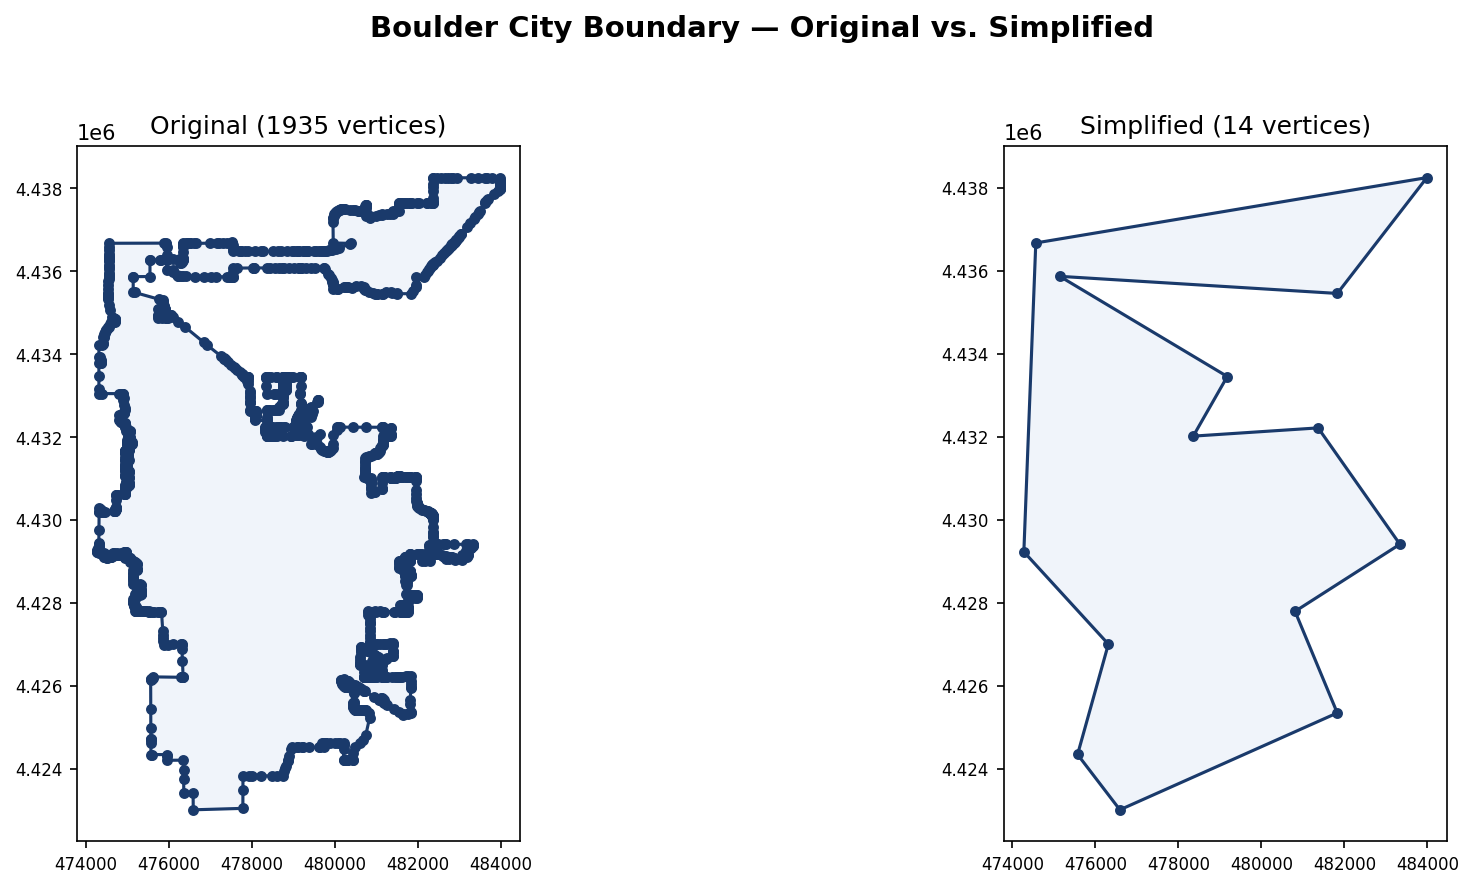
\includegraphics[width=0.82\textwidth]{figures/fig1_polygon_comparison.png}
  \caption{Left: original 1935-vertex TIGER/Line boundary of Boulder, CO
  (US Census Bureau, 2025). Right: 11-vertex simplified polygon after
  Douglas--Peucker reduction and angle smoothing, used as the domain $\Omega$
  for the SC computation. The aspect ratio and dominant geometric features are
  faithfully preserved.}
  \label{fig:poly}
\end{figure}

\subsection{Uniform Flow and the Conformal Grid}
\label{sec:res-uniform}

Figure~\ref{fig:uniform} (Appendix~\ref{app:figures}) presents the results
for uniform flow $W = U \zeta$. Streamlines ($\psi = \mathrm{const}$) enter
from the left boundary, compress through the narrow northern neck, and exit
right. Every streamline stays inside $\partial \Omega$; the no-penetration
condition holds exactly by the forward-map construction. Equipotentials
($\phi = \mathrm{const}$, Figure~\ref{fig:uniform}b) are visually orthogonal
to the streamlines throughout the interior, a consequence of the
Cauchy--Riemann equations~\eqref{eq:CR} wherever $f'(\zeta) \neq 0$
\citep[Thm.~5.4.1]{AF03}. This orthogonality is the definitive visual
confirmation of conformality. Equipotential lines alone are shown in
Figure~\ref{fig:equipotentials} (Appendix~\ref{app:figures}) for clarity.

\subsection{Terrain-Corrected Flow}

Figure~\ref{fig:terrain} (Appendix~\ref{app:figures}) shows streamlines under
the terrain potential~\eqref{eq:terrain}. Compared to the uniform baseline,
streamlines shift eastward (toward lower elevation) throughout the western
half, reproducing the slope-driven drainage pattern of Boulder's topography.
High-elevation source vertices (2057\,m, western side) push flow into the
domain; low-elevation sink vertices (1576\,m, eastern side) draw it out.
The deflection is most pronounced along the Flatirons-facing western boundary,
where the RBF-fitted elevation gradient is steepest.

\subsection{Enriched Flow Corrections: Urban Obstacle and Road Vortices}
\label{sec:res-enriched}

The urban-obstacle and road-vortex models share a common structure: both
introduce features of the physical domain (a downtown core, a network of road
intersections) by locating their pre-images in $\HH$ and inserting singularities
there, paired with real-axis images to preserve $\psi = 0$ on $\partial \HH$.

\paragraph{Urban core as interior obstacle.}
The downtown commercial core (OSMnx~\citep{BG17} landuse data, 6-vertex convex
hull, $0.82$\,km$^2$) is mapped to $\HH$ via $f^{-1}$; its pre-image is enclosed
by a circle of radius $a$ centred at $\zeta_0 \in \HH$. The Milne-Thomson
dipole in~\eqref{eq:urban} enforces no-penetration on this circle, while the
image term $U a^2 / (\bar{\zeta} - \bar{\zeta}_0)$ preserves $\psi = 0$ on $\RR$.
Figure~\ref{fig:urban} (Appendix~\ref{app:figures}) shows the resulting
potential. The achieved separation ratio $\Imag(\zeta_0) / a \approx 5.36$
gives an approximation error of about $3.5\%$. The deflection of streamlines
around the urban core is most clearly visible in Figure~\ref{fig:comparison},
panel~(c).

\paragraph{Road-vortex field.}
Of the 12 highest-degree OSM intersections (primary through tertiary roads),
11 were mapped to $\HH$; one failed near the boundary. Each intersection becomes
a point vortex in $\HH$ paired with its real-axis image, as
in~\eqref{eq:road}. Figure~\ref{fig:road} (Appendix~\ref{app:figures}) marks
CCW vortices north of the polygon centroid with orange triangles
($\Gamma > 0$) and CW vortices south with blue triangles ($\Gamma < 0$).
Local eddies are visible at each vortex; the overall CCW/CW shear pattern
approximates the vortex-pair structure of Boulder's prevailing westerly flow
regime.

\subsection{Four-Model Comparison}

Figure~\ref{fig:comparison} presents all four models side by side at
identical contour levels. The progressive physical enrichment is apparent.
Uniform flow establishes the baseline conformal grid. The terrain correction
bends streamlines eastward (downhill) throughout the western half. Panel~(c)
shows the urban obstacle creating a deflection region and a local acceleration
on the flanks of the downtown core. The road-vortex model superimposes organised
local circulation at each intersection node. Crucially, every panel is computed
from the same forward SC map and the same normalised polygon, so the only
difference between panels is the analytic form of $W(\zeta)$. This illustrates
the modular power of the conformal-mapping framework: physical complexity is
added by modifying the potential in $\HH$, rather than by re-meshing or
re-solving a PDE in $\Omega$.

\begin{figure}[tp]
  \centering
  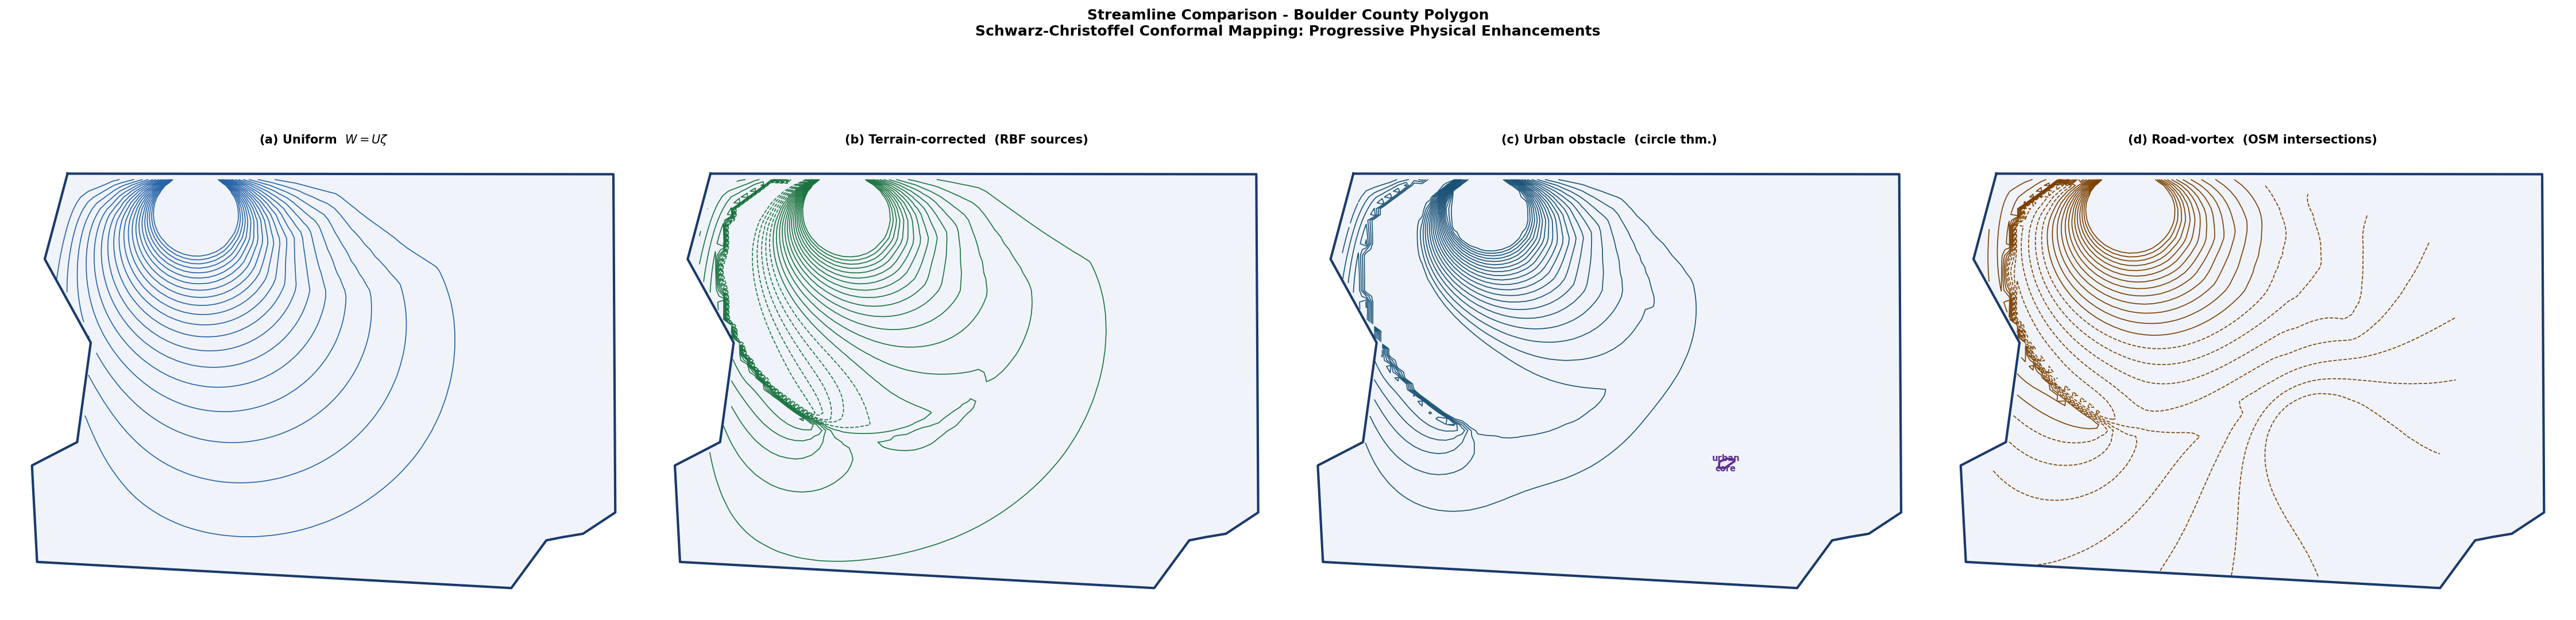
\includegraphics[width=\textwidth]{figures/fig11_four_way_comparison.png}
  \caption{Four-way comparison at identical contour levels. From left to
  right: (1) uniform flow $W = U\zeta$; (2) terrain-corrected potential
  \eqref{eq:terrain}; (3) urban-obstacle potential \eqref{eq:urban};
  (4) road-vortex potential \eqref{eq:road}. All panels share the same
  SC map $f : \HH \to \Omega$; physical enrichment is achieved by modifying
  $W(\zeta)$ in $\HH$.}
  \label{fig:comparison}
\end{figure}

\section{Conclusions and Future Directions}
\label{sec:conclusions}

We have demonstrated that the Schwarz--Christoffel transformation provides
a clean, exact framework for ideal fluid flow in an irregular polygonal domain.
The forward-map approach evaluates analytically tractable potentials in $\HH$
and maps the results to $\Omega$, yielding artifact-free streamlines that
satisfy the no-penetration condition exactly. Four physically motivated
complex potentials were derived and visualised; each extends the previous by
an additive term that preserves the boundary condition via the method of images.

The principal mathematical content is the interplay between conformal-mapping
theory (Riemann Mapping Theorem, SC integral formula, interior angle structure,
M\"obius normalisation) and ideal-flow theory (complex potential, circle theorem,
point vortices, method of images). The SC formula~\eqref{eq:SC} encodes the
polygon geometry directly through the exponents $\alpha_k - 1$: each vertex
angle appears as a branch-point strength of the integrand. The Cauchy--Riemann
equations, through the conformality of $f$, guarantee that every solution of
Laplace's equation in $\HH$ pulls back to a solution in $\Omega$; this is the
fundamental reason why conformal mapping works for fluid flow.

Numerically, the softmax reparameterisation of the pre-vertex problem transforms
a constrained optimisation into an unconstrained one, enabling
Levenberg--Marquardt to converge reliably. The forward-map approach avoids the
per-point Newton iterations of the inverse map at the cost of a scattered-data
interpolation step.

\paragraph{Future directions.}
Several extensions are natural.

\begin{itemize}[leftmargin=2em]

\item \textbf{Exact doubly-connected SC map.} The Milne-Thomson approximation
  \eqref{eq:urban} has error $O((a / \Imag\,\zeta_0)^2)$. The achieved ratio
  $\Imag(\zeta_0) / a \approx 5.36$ gives $\sim\!3.5\%$ error. An exact
  doubly-connected SC map (Driscoll--Trefethen, Chapter~5) would give a rigorous
  treatment of the doubly-connected domain.

\item \textbf{Other city shapes.} The pipeline is city-agnostic.
  Manhattan (near-rectangular) and Los Angeles (highly non-convex) would
  illustrate how the SC exponents encode shape complexity and crowding.

\item \textbf{Multiple obstacles.} The city may contain several distinct
  obstacles. The Schottky-double conformal map or an iterative circle-theorem
  application could handle multiply-connected domains of arbitrary genus.

\item \textbf{Viscous correction.} The Stokes stream function satisfies a
  biharmonic equation $\nabla^4 \psi = 0$. Comparing ideal and Stokes streamlines
  would quantify the effect of viscosity near the boundary.

\item \textbf{Time-dependent flow.} Adding a time-dependent circulation
  $\Gamma(t)$ around the domain or obstacle would model unsteady effects
  such as gust events, which are common in Boulder's complex terrain.

\end{itemize}

\bibliography{refs}

\clearpage
\appendix
\section{Supplementary Figures}
\label{app:figures}

Per-model results referenced in Section~\ref{sec:results} are collected here,
followed by supplementary comparison panels. Detailed interpretation is given
in the main body; captions below are brief labels.

\begin{figure}[H]
  \centering
  \begin{subfigure}[b]{0.48\textwidth}
    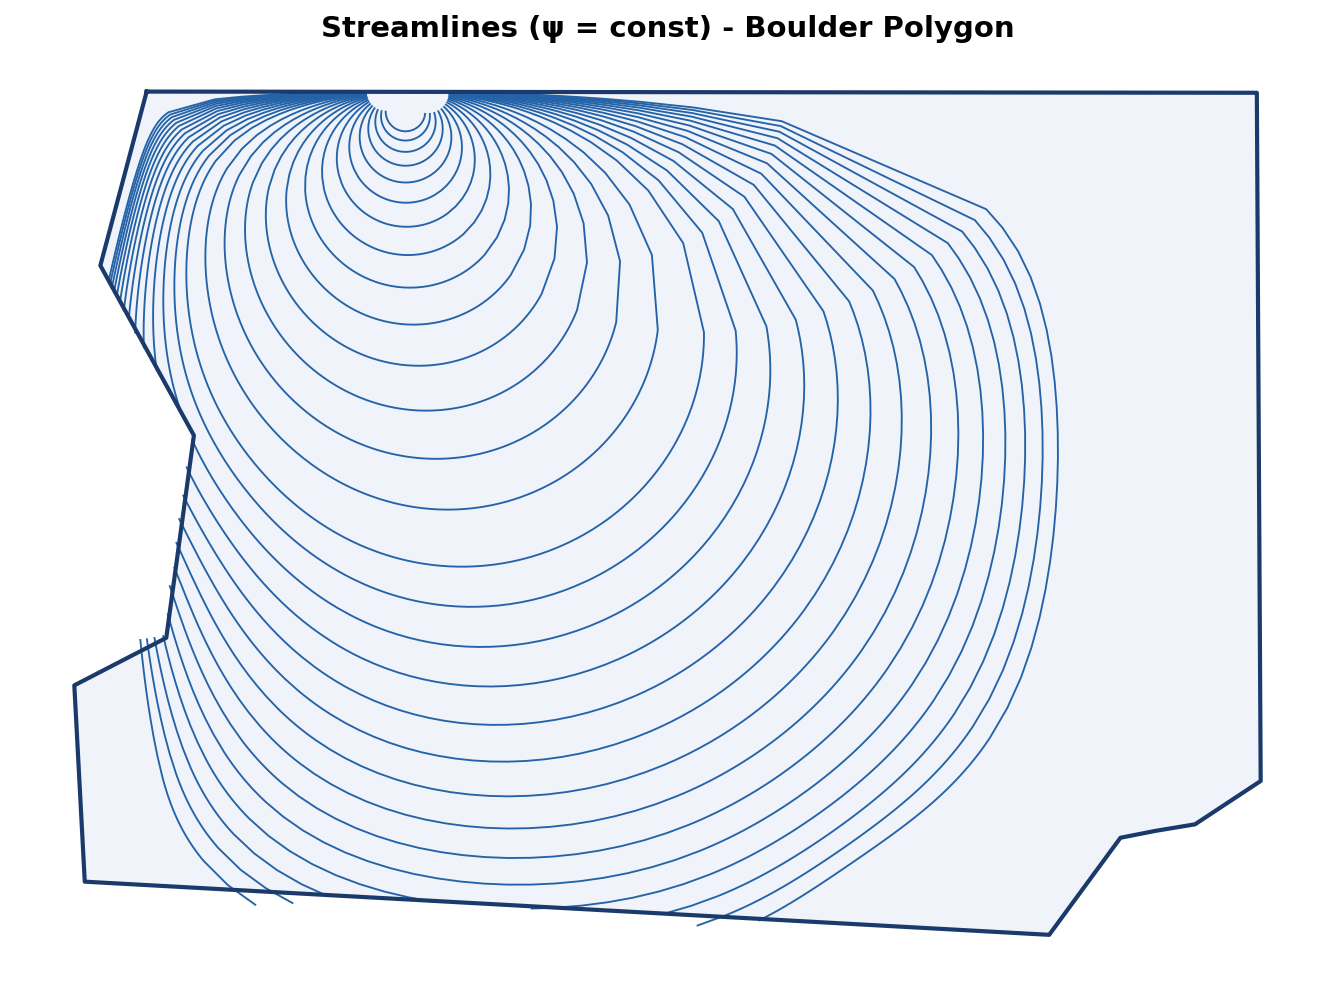
\includegraphics[width=\textwidth]{figures/fig2_streamlines.png}
    \caption{Streamlines $\psi = \mathrm{const}$.}
  \end{subfigure}\hfill
  \begin{subfigure}[b]{0.48\textwidth}
    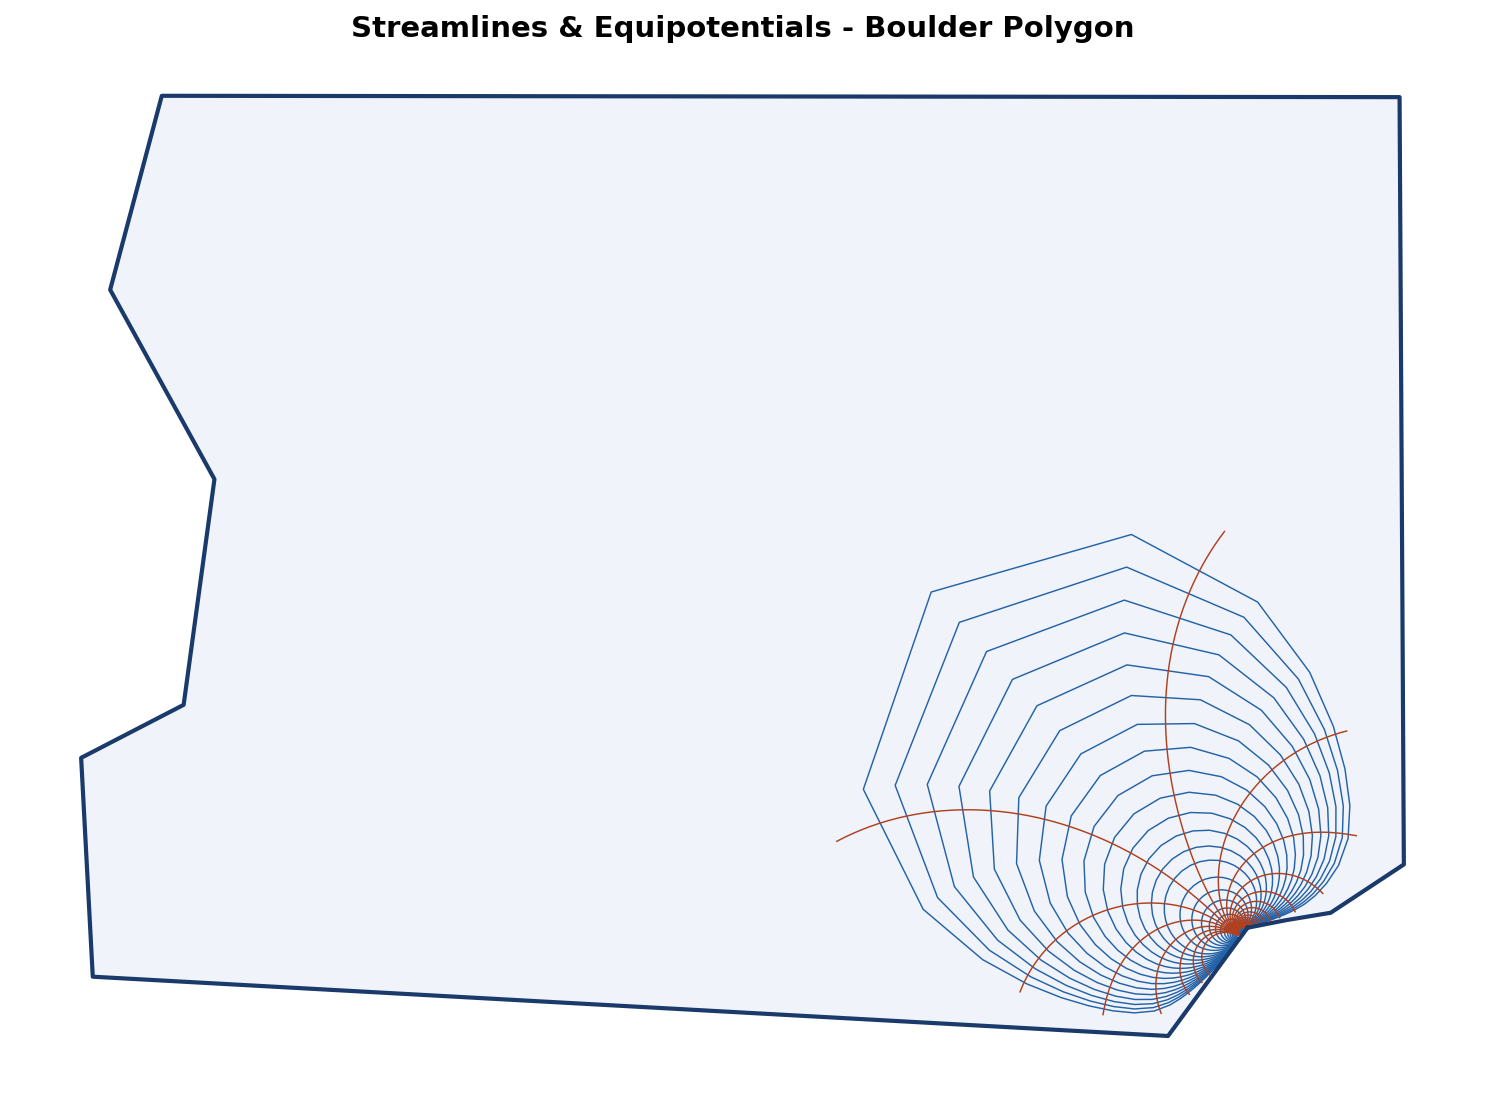
\includegraphics[width=\textwidth]{figures/fig4_combined.png}
    \caption{Conformal grid: streamlines + equipotentials.}
  \end{subfigure}
  \caption{Uniform flow $W = U\zeta$ in $\Omega$. See Section~\ref{sec:res-uniform}.}
  \label{fig:uniform}
\end{figure}

\begin{figure}[H]
  \centering
  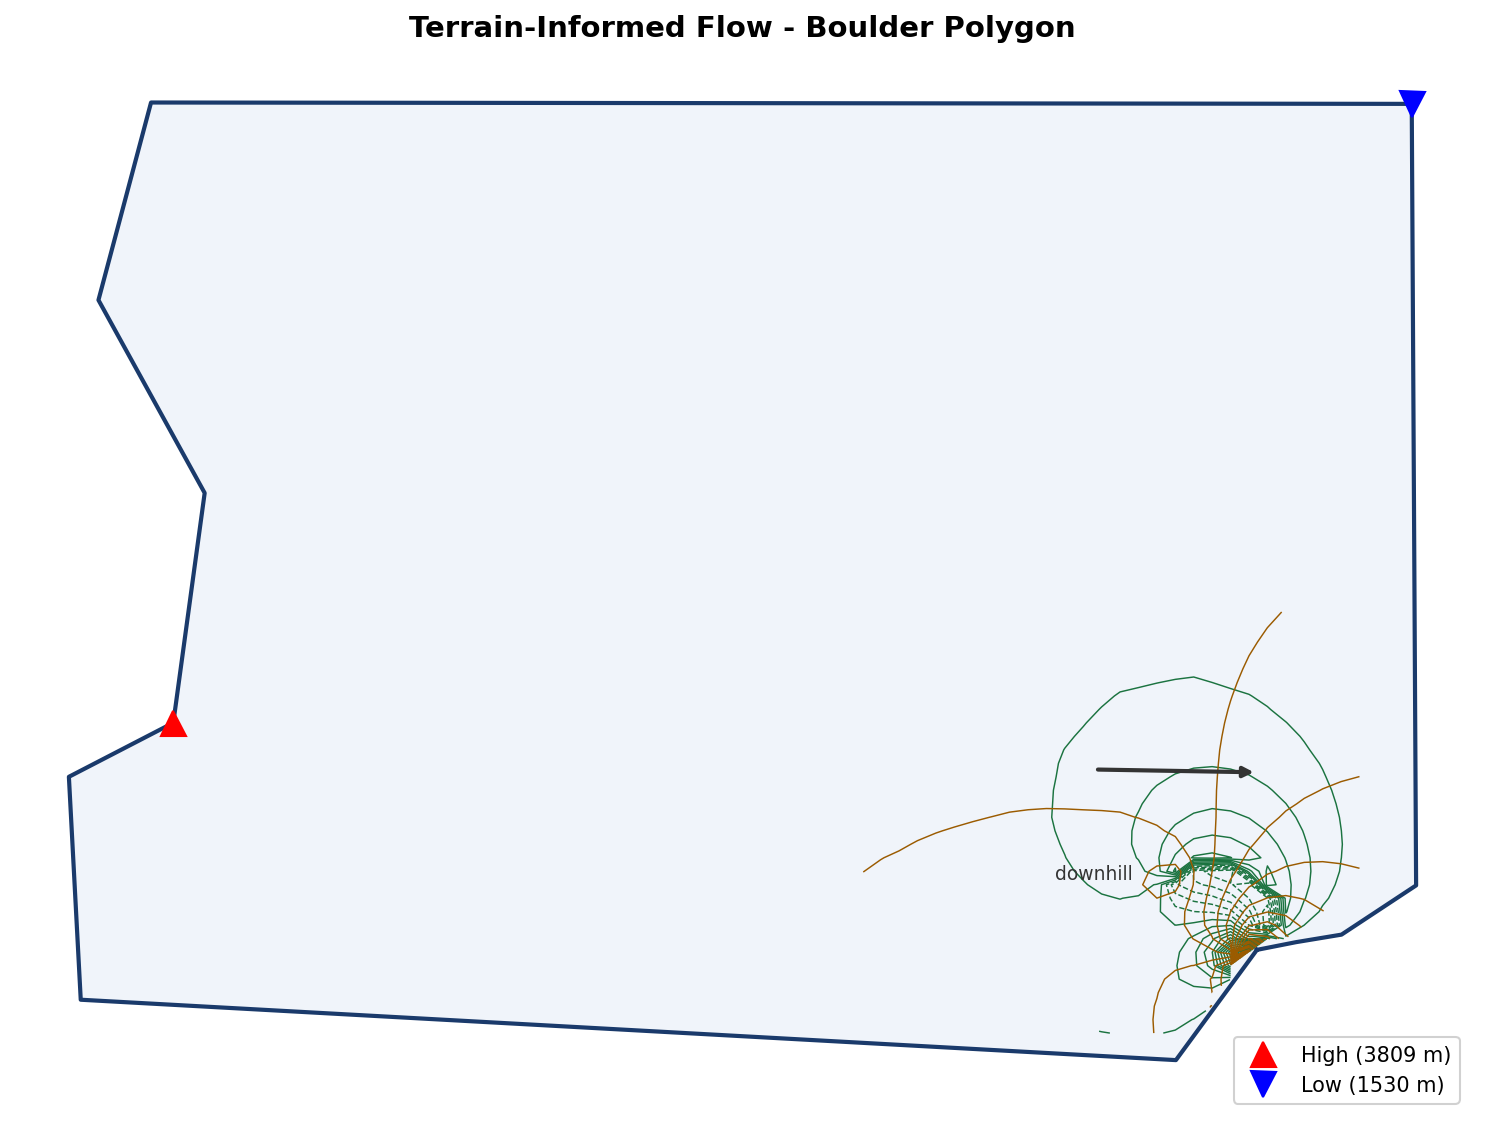
\includegraphics[width=0.65\textwidth]{figures/fig5_terrain_flow.png}
  \caption{Terrain-corrected potential~\eqref{eq:terrain}: streamlines (green),
  equipotentials (amber), high-elevation sources (red triangles), low-elevation
  sinks (blue triangles).}
  \label{fig:terrain}
\end{figure}

\begin{figure}[H]
  \centering
  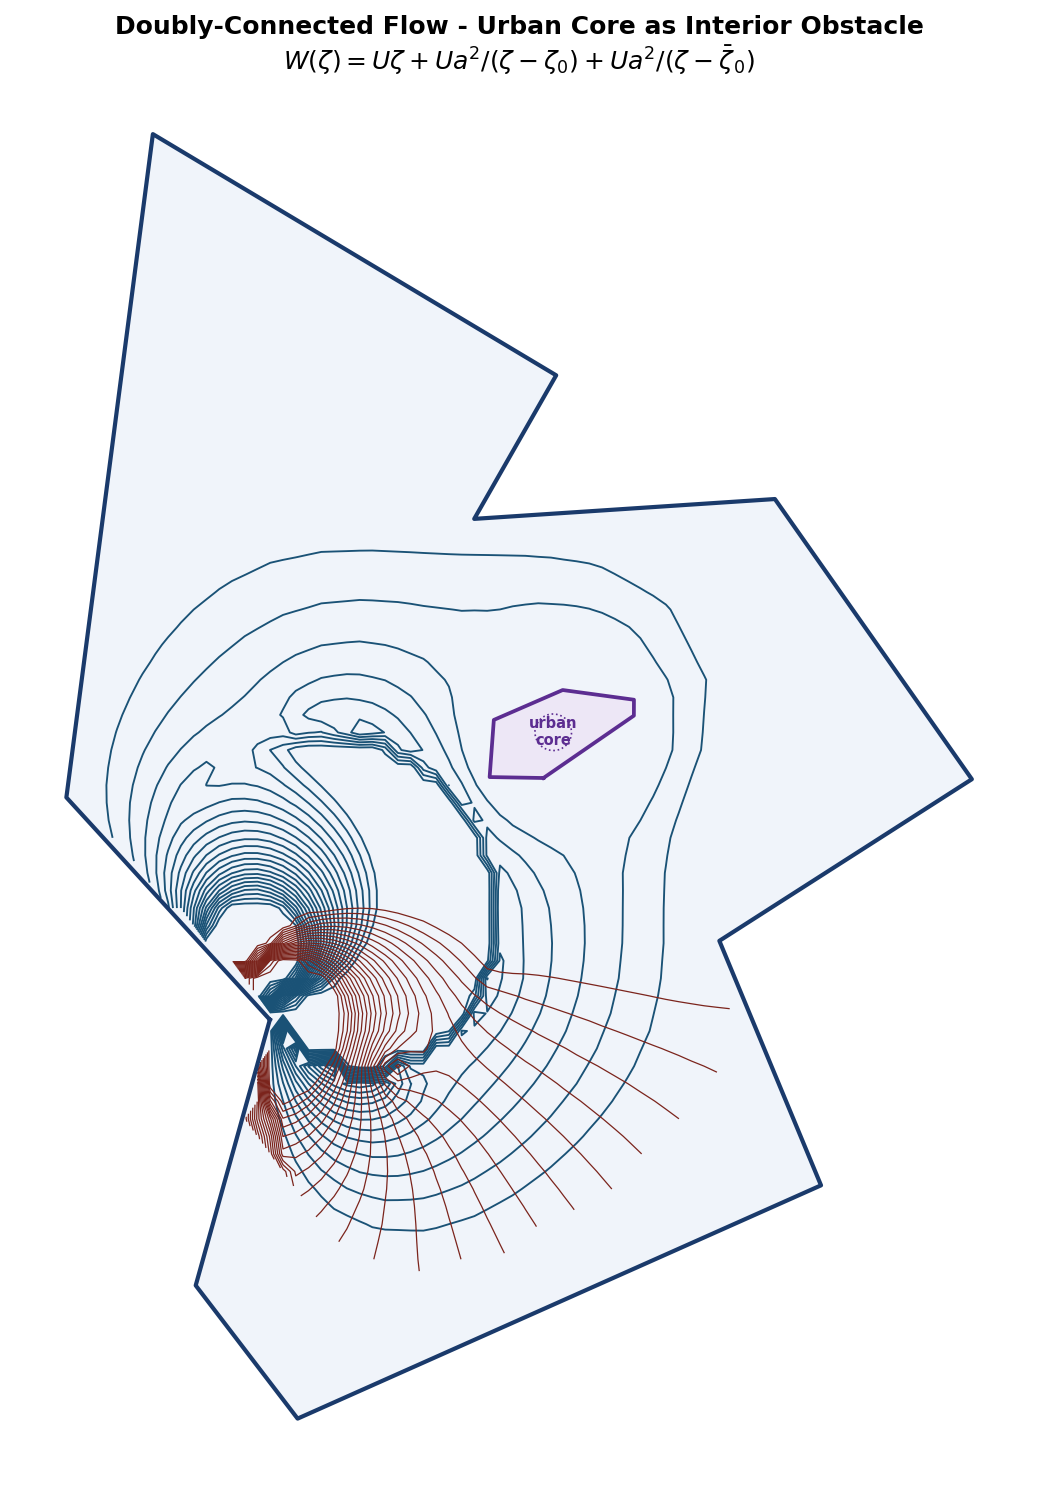
\includegraphics[width=0.65\textwidth]{figures/fig7_urban_flow.png}
  \caption{Urban-obstacle potential~\eqref{eq:urban}. Downtown core shown in
  purple. Separation ratio $\Imag(\zeta_0)/a \approx 5.36$.}
  \label{fig:urban}
\end{figure}

\begin{figure}[H]
  \centering
  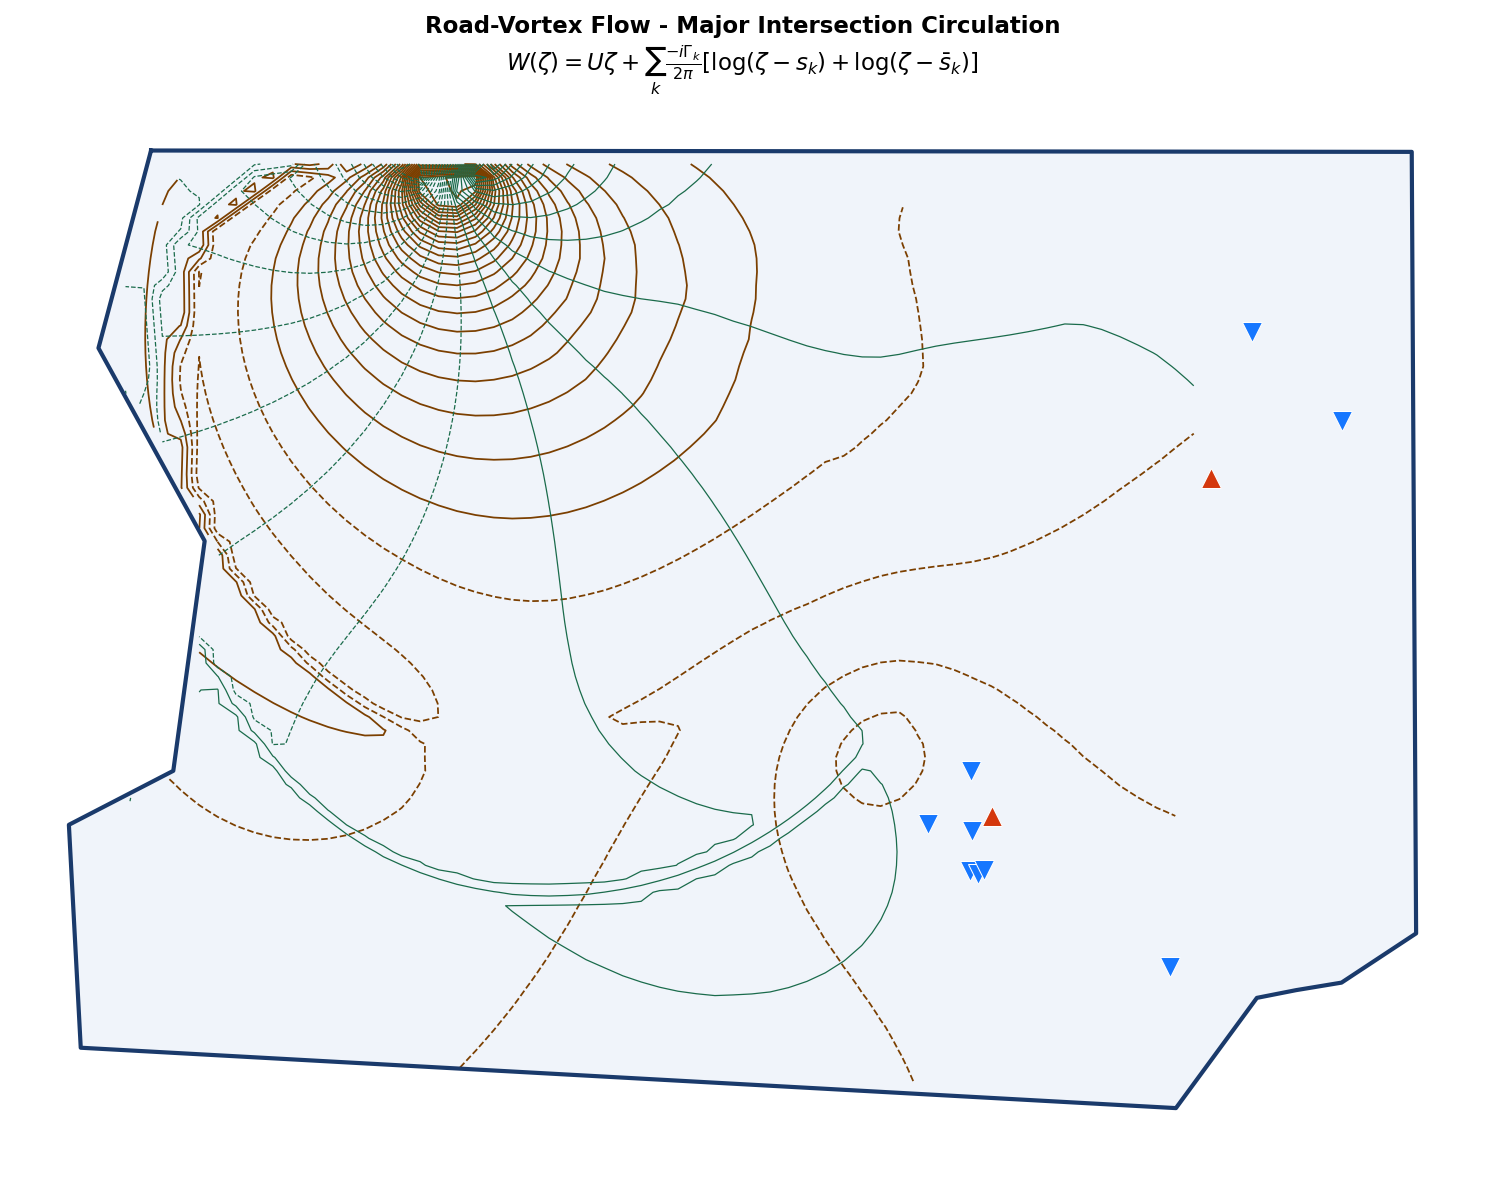
\includegraphics[width=0.65\textwidth]{figures/fig9_road_flow.png}
  \caption{Road-vortex potential~\eqref{eq:road}. Orange triangles:
  $\Gamma > 0$ (CCW, north of centroid). Blue triangles: $\Gamma < 0$ (CW, south).}
  \label{fig:road}
\end{figure}

\begin{figure}[H]
  \centering
  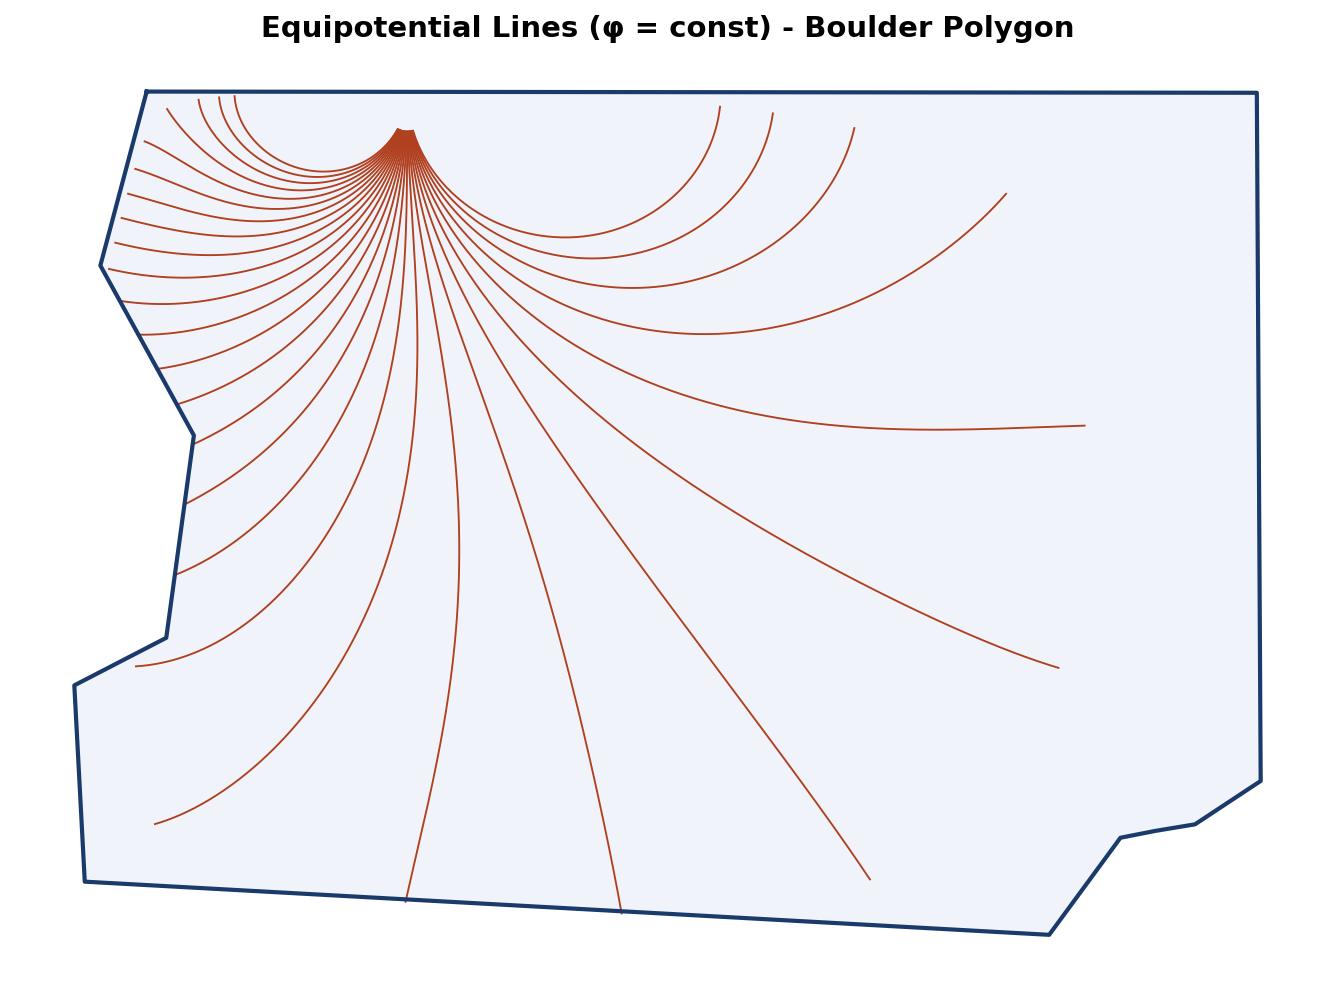
\includegraphics[width=0.72\textwidth]{figures/fig3_equipotentials.png}
  \caption{Equipotentials $\phi = \mathrm{const}$ for uniform flow, shown alone.}
  \label{fig:equipotentials}
\end{figure}

\begin{figure}[H]
  \centering
  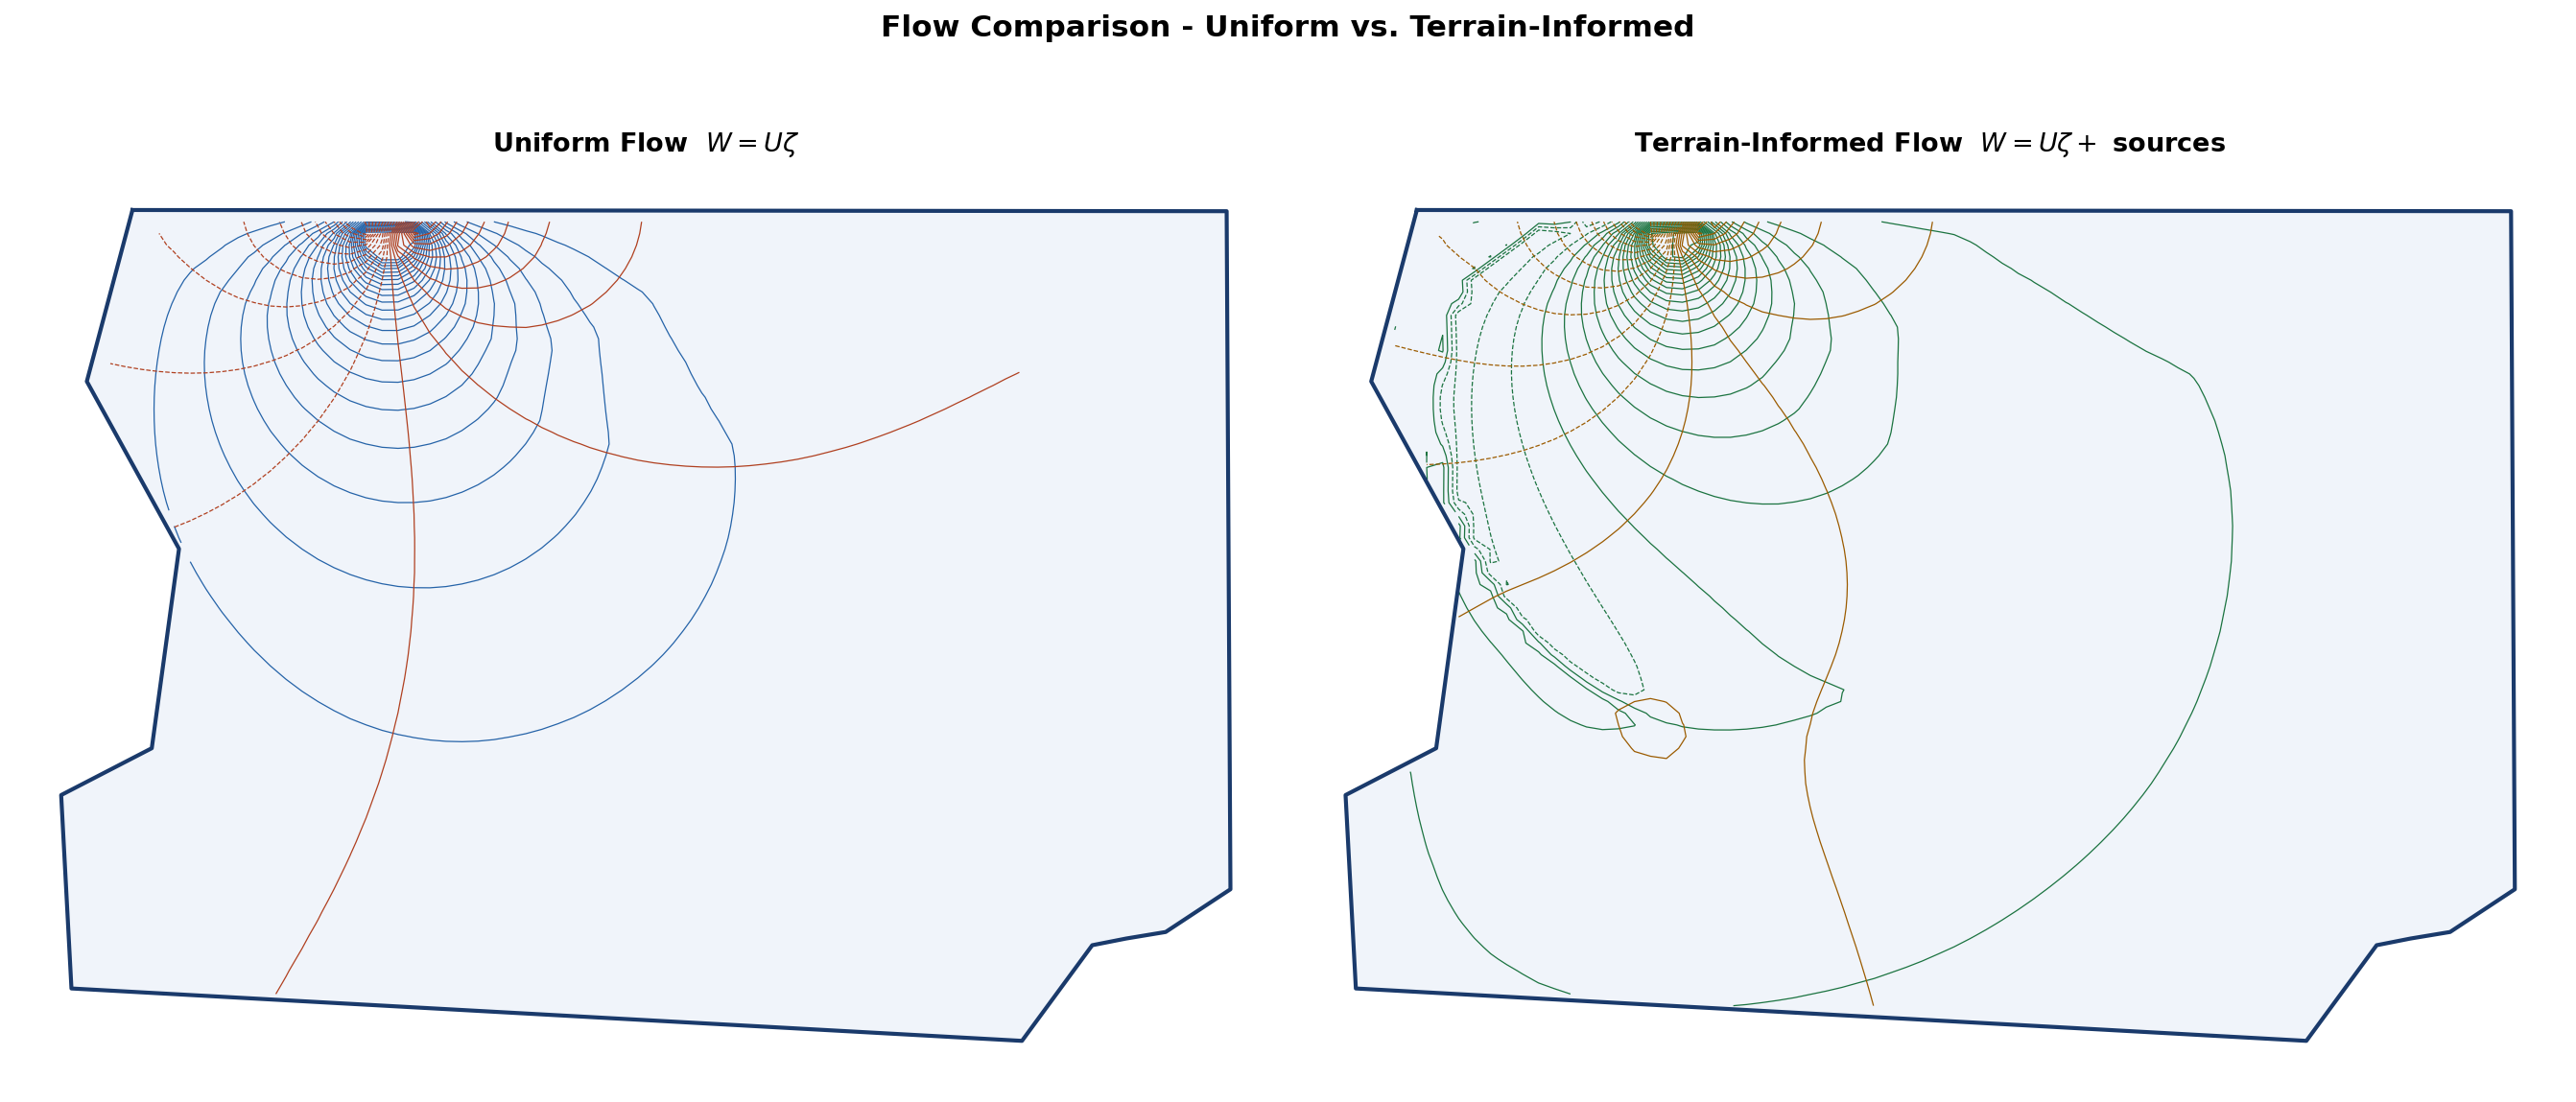
\includegraphics[width=0.88\textwidth]{figures/fig6_flow_comparison.png}
  \caption{Uniform flow (left) vs.\ terrain-corrected flow (right).}
  \label{fig:terrain_compare}
\end{figure}

\begin{figure}[H]
  \centering
  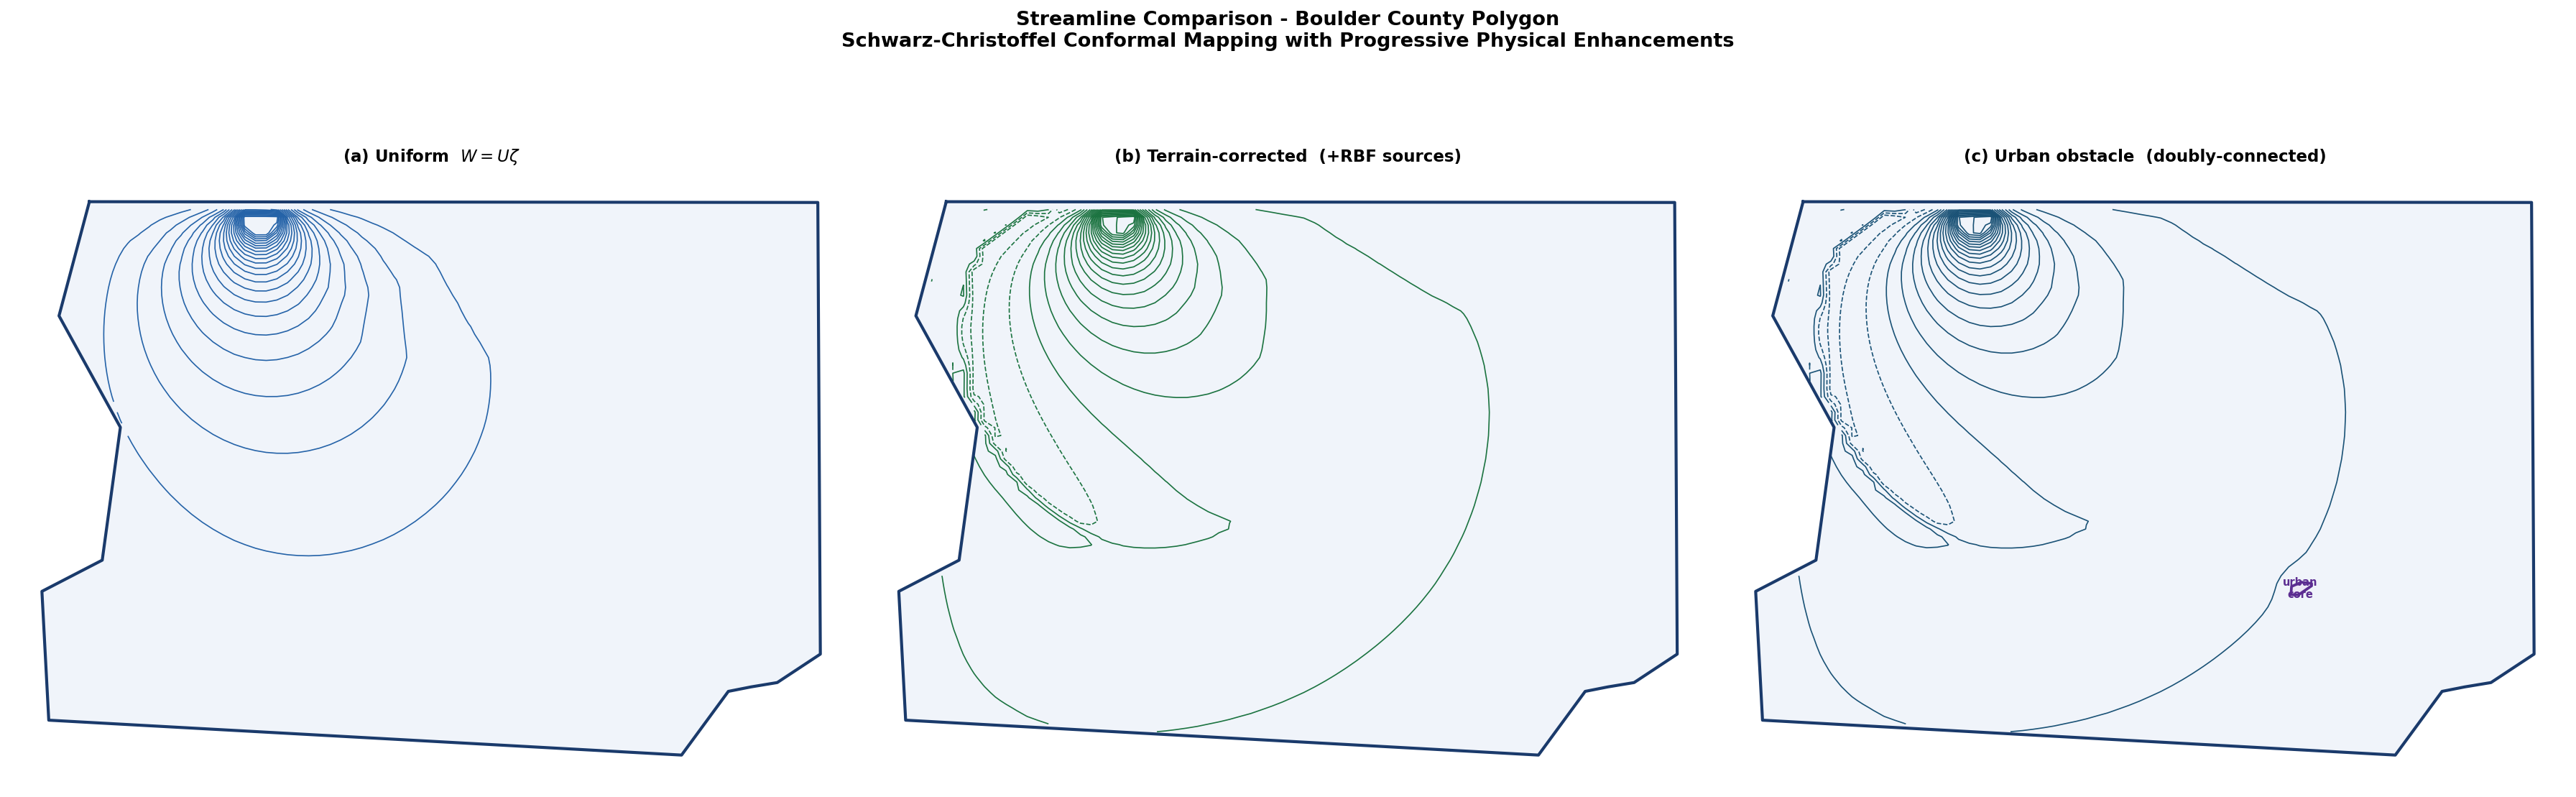
\includegraphics[width=\textwidth]{figures/fig8_three_way_comparison.png}
  \caption{Three-way comparison: uniform, terrain-corrected, urban-obstacle.}
  \label{fig:three_way}
\end{figure}

\begin{figure}[H]
  \centering
  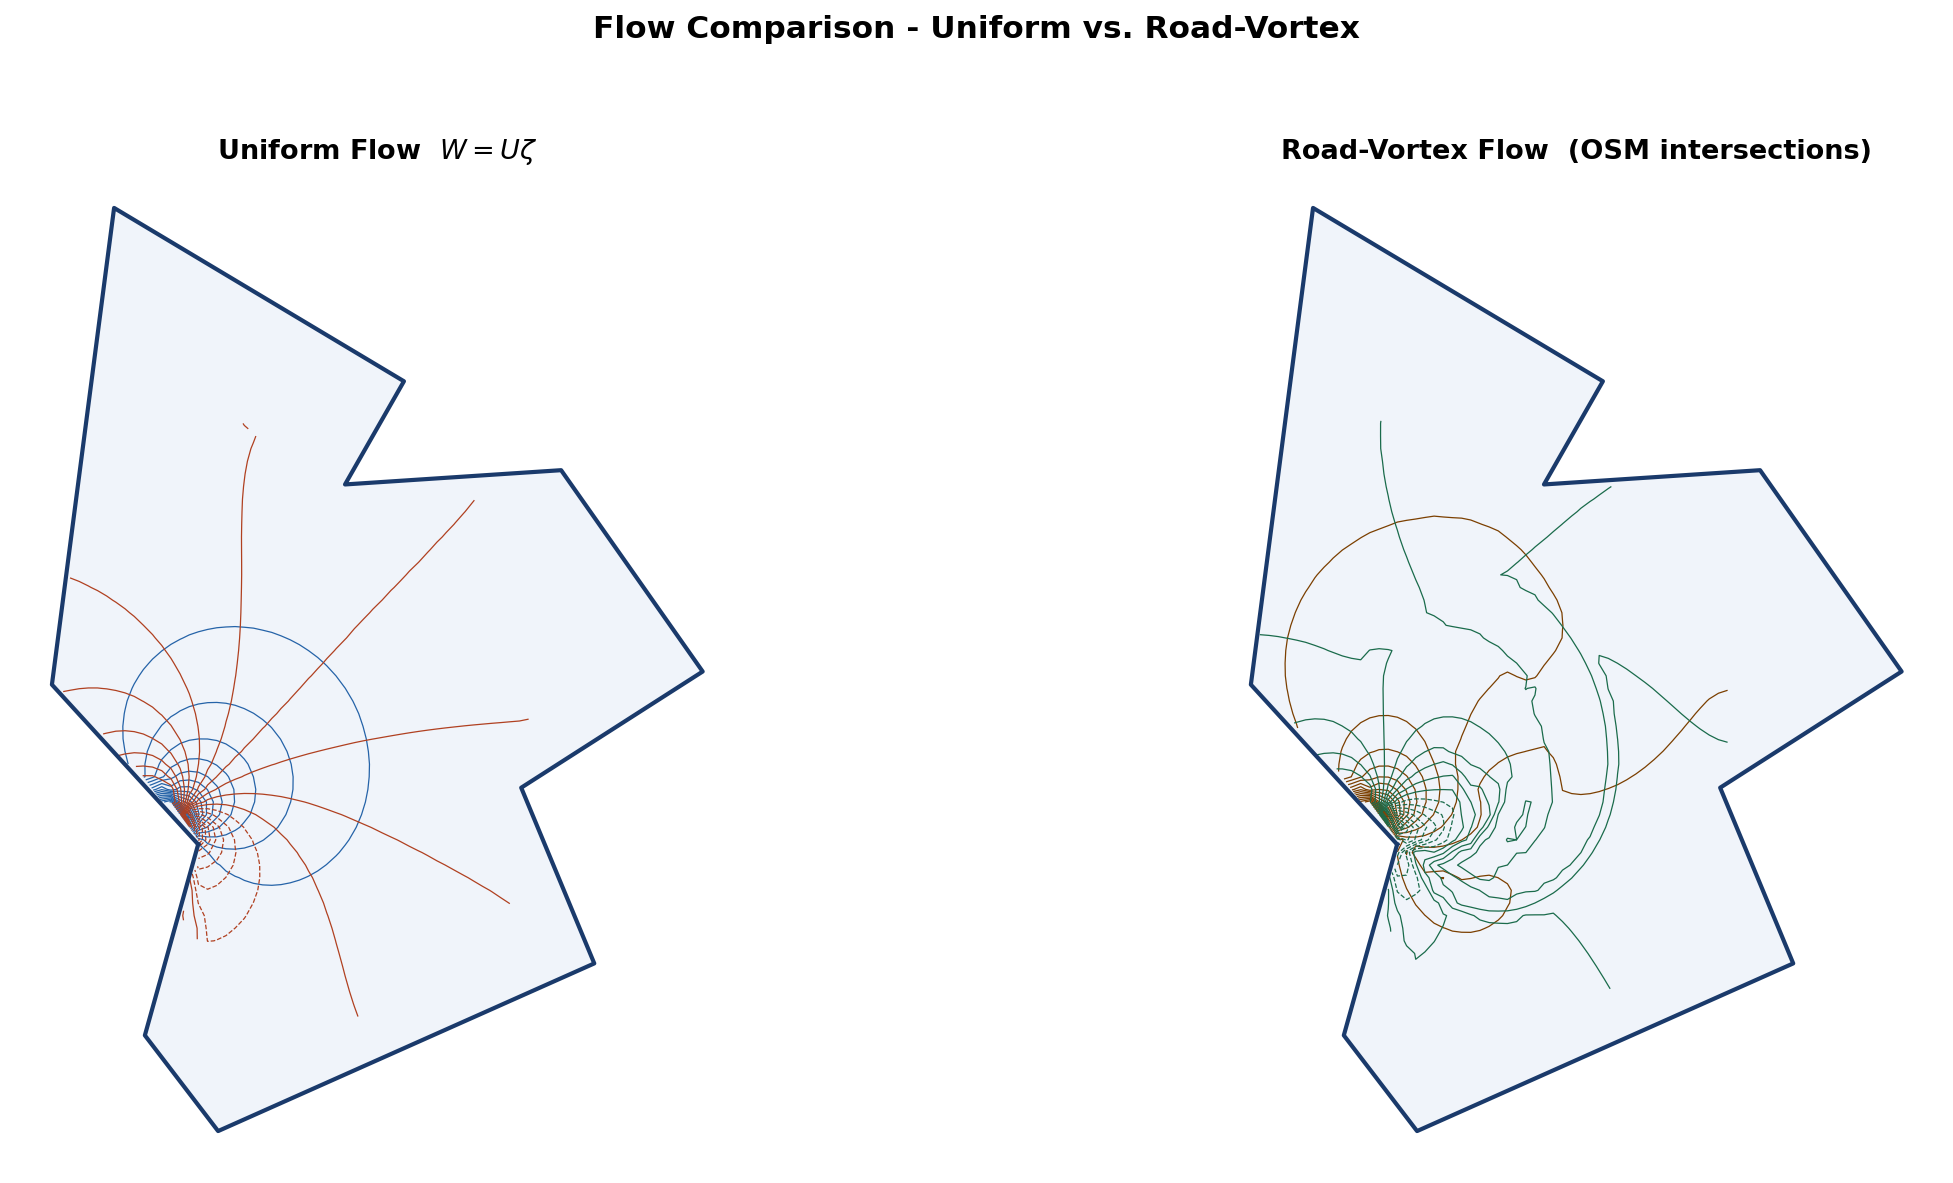
\includegraphics[width=0.88\textwidth]{figures/fig10_road_vs_uniform.png}
  \caption{Uniform flow (left) vs.\ road-vortex flow (right).}
  \label{fig:road_compare}
\end{figure}

\section{Code and Reproducibility}
\label{app:code}

All source code is publicly available at
\url{https://github.com/McDonaldCrispyThigh/Ideal-Flow-via-Schwarz-Christoffel}.
The full pipeline is reproduced by:
\begin{verbatim}
  pip install -r requirements.txt
  python main.py --shapefile data/raw/tl_2025_08_place \
                 --terrain --urban --roads --grid 80
\end{verbatim}
Key modules: \texttt{src/polygon.py} (boundary preprocessing),
\texttt{src/angles.py} (interior angle computation),
\texttt{src/sc\_solver.py} (SC parameter problem, Gauss--Legendre quadrature,
forward map),
\texttt{src/terrain.py} (USGS 3DEP API, RBF surface, per-vertex sources),
\texttt{src/urban.py} (OSM obstacle, Welzl minimum enclosing circle),
\texttt{src/roads.py} (OSM road intersections, SC inverse map, vortex placement),
\texttt{src/sc\_solver\_dc.py} (combined potentials), and
\texttt{src/visualization.py} (publication-quality figures).

\noindent\textbf{Software:} Python~3.14, NumPy~2.2, SciPy~1.15,
Shapely~2.0, GeoPandas~1.0, OSMnx~2.0~\citep{BG17}, Matplotlib~3.10,
pyproj~3.7, tqdm~4.67.

\end{document}
